        %%******************************************%%
        %%                                          %%
        %%        Modello di tesi di laurea         %%
        %%            di Andrea Giraldin            %%
        %%                                          %%
        %%             2 novembre 2012              %%
        %%                                          %%
        %%******************************************%%


% I seguenti commenti speciali impostano:
% 1. 
% 2. PDFLaTeX come motore di composizione;
% 3. tesi.tex come documento principale;
% 4. il controllo ortografico italiano per l'editor.

% !TEX encoding = UTF-8
% !TEX TS-program = pdflatex
% !TEX root = tesi.tex
% !TEX spellcheck = it-IT

% PDF/A filecontents
\RequirePackage{filecontents}
\begin{filecontents*}{\jobname.xmpdata}
  \Title{Containerization \& Distribution of Game Engines}
  \Author{Alessandro Sgreva}
  \Language{en-GB}
  \Subject{Containerization \& Distribution of Game Engines}
  \Keywords{containerization\sep Distribution\sep Game\sep Engines\sep}
\end{filecontents*}

\documentclass[10pt,                    % corpo del font principale
               a4paper,                 % carta A4
               twoside,                 % impagina per fronte-retro
               openright,               % inizio capitoli a destra
               english,                                  
               ]{book}    

%**************************************************************
% Importazione package
%************************************************************** 

\PassOptionsToPackage{table, dvipsnames}{xcolor} % colori PDF/A

\usepackage{lscape}

\usepackage[T1]{fontenc}

\usepackage{lmodern}

\usepackage{colorprofiles}

\usepackage[a-2b,mathxmp]{pdfx}[2018/12/22]
                                        % configurazione PDF/A
                                        % validare in https://www.pdf-online.com/osa/validate.aspx

%\usepackage{amsmath,amssymb,amsthm}    % matematica

\usepackage[T1]{fontenc}                % codifica dei font:
                                        % NOTA BENE! richiede una distribuzione *completa* di LaTeX

\usepackage[utf8]{inputenc}             % codifica di input; anche [latin1] va bene
                                        % NOTA BENE! va accordata con le preferenze dell'editor

\usepackage[english]{babel}    % per scrivere in italiano e in inglese;
                                        % l'ultima lingua (l'italiano) risulta predefinita

\usepackage{bookmark}                   % segnalibri

\usepackage{caption}                    % didascalie

\usepackage{chngpage,calc}              % centra il frontespizio

\usepackage{csquotes}                   % gestisce automaticamente i caratteri (")

\usepackage{emptypage}                  % pagine vuote senza testatina e piede di pagina

\usepackage{epigraph}			% per epigrafi

\usepackage{eurosym}                    % simbolo dell'euro

%\usepackage{indentfirst}               % rientra il primo paragrafo di ogni sezione

\usepackage{graphicx}                   % immagini

\usepackage{hyperref}                   % collegamenti ipertestuali

\usepackage[binding=5mm]{layaureo}      % margini ottimizzati per l'A4; rilegatura di 5 mm

\usepackage{listings}                   % codici

\usepackage{microtype}                  % microtipografia

\usepackage{mparhack,fixltx2e,relsize}  % finezze tipografiche

\usepackage{nameref}                    % visualizza nome dei riferimenti                                      
\usepackage[font=small]{quoting}        % citazioni

\usepackage{subfig}                     % sottofigure, sottotabelle

\usepackage[english]{varioref}          % riferimenti completi della pagina

\usepackage{booktabs}                   % tabelle                                       
\usepackage{tabularx}                   % tabelle di larghezza prefissata                                    
\usepackage{longtable}                  % tabelle su più pagine                                        
\usepackage{ltxtable}                   % tabelle su più pagine e adattabili in larghezza

\usepackage[toc, acronym]{glossaries}   % glossario
                                        % per includerlo nel documento bisogna:
                                        % 1. compilare una prima volta tesi.tex;
                                        % 2. eseguire: makeindex -s tesi.ist -t tesi.glg -o tesi.gls tesi.glo
                                        % 3. eseguire: makeindex -s tesi.ist -t tesi.alg -o tesi.acr tesi.acn
                                        % 4. compilare due volte tesi.tex.

\usepackage[defernumbers=true,style=numeric-comp,useprefix,hyperref,backend=bibtex]{biblatex}
                                        % eccellente pacchetto per la bibliografia; 
                                        % produce uno stile di citazione autore-anno; 
                                        % lo stile "numeric-comp" produce riferimenti numerici
                                        % per includerlo nel documento bisogna:
                                        % 1. compilare una prima volta tesi.tex;
                                        % 2. eseguire: biber tesi
                                        % 3. compilare ancora tesi.tex.

%**************************************************************
% file contenente le impostazioni della tesi
%**************************************************************

%**************************************************************
% Frontespizio
%**************************************************************

% Autore
\newcommand{\myName}{Riccardo Montagnin}                                    
\newcommand{\myTitle}{Titolo della tesi}

% Tipo di tesi                   
\newcommand{\myDegree}{Tesi di laurea}

% Università             
\newcommand{\myUni}{Università degli Studi di Padova}

% Facoltà       
\newcommand{\myFaculty}{Corso di Laurea in Informatica}

% Dipartimento
\newcommand{\myDepartment}{Dipartimento di Matematica "Tullio Levi-Civita"}

% Titolo del relatore
\newcommand{\profTitle}{Prof.}

% Relatore
\newcommand{\myProf}{Tullio Vardanega}

% Luogo
\newcommand{\myLocation}{Padova}

% Anno accademico
\newcommand{\myAA}{2016-2017}

% Data discussione
\newcommand{\myTime}{Luglio 2017}


%**************************************************************
% Impostazioni di impaginazione
% see: http://wwwcdf.pd.infn.it/AppuntiLinux/a2547.htm
%**************************************************************

\setlength{\parindent}{14pt}   % larghezza rientro della prima riga
\setlength{\parskip}{0pt}   % distanza tra i paragrafi


%**************************************************************
% Impostazioni di biblatex
%**************************************************************
\bibliography{bibliografia} % database di biblatex 

\defbibheading{bibliography} {
    \cleardoublepage
    \phantomsection 
    \addcontentsline{toc}{chapter}{\bibname}
    \chapter*{\bibname\markboth{\bibname}{\bibname}}
}

\setlength\bibitemsep{1.5\itemsep} % spazio tra entry

\DeclareBibliographyCategory{opere}
\DeclareBibliographyCategory{web}

\addtocategory{opere}{womak:lean-thinking}
\addtocategory{web}{site:agile-manifesto}

\defbibheading{opere}{\section*{Riferimenti bibliografici}}
\defbibheading{web}{\section*{Siti Web consultati}}


%**************************************************************
% Impostazioni di caption
%**************************************************************
\captionsetup{
    tableposition=top,
    figureposition=bottom,
    font=small,
    format=hang,
    labelfont=bf
}

%**************************************************************
% Impostazioni di glossaries
%**************************************************************

%**************************************************************
% Acronimi
%**************************************************************
\renewcommand{\acronymname}{Acronimi e abbreviazioni}

\newacronym[description={\glslink{apig}{Application Program Interface}}]
    {api}{API}{Application Program Interface}

\newacronym[description={\glslink{umlg}{Unified Modeling Language}}]
    {uml}{UML}{Unified Modeling Language}

%**************************************************************
% Glossario
%**************************************************************
%\renewcommand{\glossaryname}{Glossario}

\newglossaryentry{apig}
{
    name=\glslink{api}{API},
    text=Application Program Interface,
    sort=api,
    description={in informatica con il termine \emph{Application Programming Interface API} (ing. interfaccia di programmazione di un'applicazione) si indica ogni insieme di procedure disponibili al programmatore, di solito raggruppate a formare un set di strumenti specifici per l'espletamento di un determinato compito all'interno di un certo programma. La finalità è ottenere un'astrazione, di solito tra l'hardware e il programmatore o tra software a basso e quello ad alto livello semplificando così il lavoro di programmazione}
}

\newglossaryentry{umlg}
{
    name=\glslink{uml}{UML},
    text=UML,
    sort=uml,
    description={in ingegneria del software \emph{UML, Unified Modeling Language} (ing. linguaggio di modellazione unificato) è un linguaggio di modellazione e specifica basato sul paradigma object-oriented. L'\emph{UML} svolge un'importantissima funzione di ``lingua franca'' nella comunità della progettazione e programmazione a oggetti. Gran parte della letteratura di settore usa tale linguaggio per descrivere soluzioni analitiche e progettuali in modo sintetico e comprensibile a un vasto pubblico}
}
 % database di termini
\makeglossaries


%**************************************************************
% Impostazioni di graphicx
%**************************************************************
\graphicspath{{immagini/}} % cartella dove sono riposte le immagini


%**************************************************************
% Impostazioni di hyperref
%**************************************************************
\hypersetup{
    %hyperfootnotes=false,
    %pdfpagelabels,
    %draft,	% = elimina tutti i link (utile per stampe in bianco e nero)
    colorlinks=true,
    linktocpage=true,
    pdfstartpage=1,
    pdfstartview=,
    % decommenta la riga seguente per avere link in nero (per esempio per la stampa in bianco e nero)
    %colorlinks=false, linktocpage=false, pdfborder={0 0 0}, pdfstartpage=1, pdfstartview=FitV,
    breaklinks=true,
    pdfpagemode=UseNone,
    pageanchor=true,
    pdfpagemode=UseOutlines,
    plainpages=false,
    bookmarksnumbered,
    bookmarksopen=true,
    bookmarksopenlevel=1,
    hypertexnames=true,
    pdfhighlight=/O,
    %nesting=true,
    %frenchlinks,
    urlcolor=webbrown,
    linkcolor=RoyalBlue,
    citecolor=webgreen,
    %pagecolor=RoyalBlue,
    %urlcolor=Black, linkcolor=Black, citecolor=Black, %pagecolor=Black,
    pdftitle={\myTitle},
    pdfauthor={\textcopyright\ \myName, \myUni, \myFaculty},
    pdfsubject={},
    pdfkeywords={},
    pdfcreator={pdfLaTeX},
    pdfproducer={LaTeX}
}

%**************************************************************
% Impostazioni di itemize
%**************************************************************
\renewcommand{\labelitemi}{$\ast$}

%\renewcommand{\labelitemi}{$\bullet$}
%\renewcommand{\labelitemii}{$\cdot$}
%\renewcommand{\labelitemiii}{$\diamond$}
%\renewcommand{\labelitemiv}{$\ast$}


%**************************************************************
% Impostazioni di listings
%**************************************************************
\lstset{
    language=[LaTeX]Tex,%C++,
    keywordstyle=\color{RoyalBlue}, %\bfseries,
    basicstyle=\small\ttfamily,
    %identifierstyle=\color{NavyBlue},
    commentstyle=\color{Green}\ttfamily,
    stringstyle=\rmfamily,
    numbers=none, %left,%
    numberstyle=\scriptsize, %\tiny
    stepnumber=5,
    numbersep=8pt,
    showstringspaces=false,
    breaklines=true,
    frameround=ftff,
    frame=single
} 


%**************************************************************
% Impostazioni di xcolor
%**************************************************************
\definecolor{webgreen}{rgb}{0,.5,0}
\definecolor{webbrown}{rgb}{.6,0,0}


%**************************************************************
% Altro
%**************************************************************

\newcommand{\omissis}{[\dots\negthinspace]} % produce [...]

% eccezioni all'algoritmo di sillabazione
\hyphenation
{
    ma-cro-istru-zio-ne
    gi-ral-din
}

\newcommand{\sectionname}{sezione}
\addto\captionsitalian{\renewcommand{\figurename}{Figura}
                       \renewcommand{\tablename}{Tabella}}

\newcommand{\glsfirstoccur}{\ap{{[g]}}}

\newcommand{\intro}[1]{\emph{\textsf{#1}}}

%**************************************************************
% Environment per ``rischi''
%**************************************************************
\newcounter{riskcounter}                % define a counter
\setcounter{riskcounter}{0}             % set the counter to some initial value

%%%% Parameters
% #1: Title
\newenvironment{risk}[1]{
    \refstepcounter{riskcounter}        % increment counter
    \par \noindent                      % start new paragraph
    \textbf{\arabic{riskcounter}. #1}   % display the title before the 
                                        % content of the environment is displayed 
}{
    \par\medskip
}

\newcommand{\riskname}{Rischio}

\newcommand{\riskdescription}[1]{\textbf{\\Descrizione:} #1.}

\newcommand{\risksolution}[1]{\textbf{\\Soluzione:} #1.}

%**************************************************************
% Environment per ``use case''
%**************************************************************
\newcounter{usecasecounter}             % define a counter
\setcounter{usecasecounter}{0}          % set the counter to some initial value

%%%% Parameters
% #1: ID
% #2: Nome
\newenvironment{usecase}[2]{
    \renewcommand{\theusecasecounter}{\usecasename #1}  % this is where the display of 
                                                        % the counter is overwritten/modified
    \refstepcounter{usecasecounter}             % increment counter
    \vspace{10pt}
    \par \noindent                              % start new paragraph
    {\large \textbf{\usecasename #1: #2}}       % display the title before the 
                                                % content of the environment is displayed 
    \medskip
}{
    \medskip
}

\newcommand{\usecasename}{UC}

\newcommand{\usecaseactors}[1]{\textbf{\\Attori Principali:} #1. \vspace{4pt}}
\newcommand{\usecasepre}[1]{\textbf{\\Precondizioni:} #1. \vspace{4pt}}
\newcommand{\usecasedesc}[1]{\textbf{\\Descrizione:} #1. \vspace{4pt}}
\newcommand{\usecasepost}[1]{\textbf{\\Postcondizioni:} #1. \vspace{4pt}}
\newcommand{\usecasealt}[1]{\textbf{\\Scenario Alternativo:} #1. \vspace{4pt}}

%**************************************************************
% Environment per ``namespace description''
%**************************************************************

\newenvironment{namespacedesc}{
    \vspace{10pt}
    \par \noindent                              % start new paragraph
    \begin{description} 
}{
    \end{description}
    \medskip
}

\newcommand{\classdesc}[2]{\item[\textbf{#1:}] #2}
                     % file con le impostazioni personali

\begin{document}
%**************************************************************
% Materiale iniziale
%**************************************************************
\frontmatter
% !TEX encoding = UTF-8
% !TEX TS-program = pdflatex
% !TEX root = ../tesi.tex

%**************************************************************
% Frontespizio 
%**************************************************************
\begin{titlepage}

\begin{center}

\begin{LARGE}
\textbf{\myUni}\\
\end{LARGE}

\vspace{10pt}

\begin{Large}
\textsc{\myDepartment}\\
\end{Large}

\vspace{10pt}

\begin{large}
\textsc{\myFaculty}\\
\end{large}

\vspace{30pt}
\begin{figure}[htbp]
\begin{center}

\includegraphics[height=6cm]{logo-unipd}
\end{center}
\end{figure}
\vspace{30pt} 

\begin{LARGE}
\begin{center}
\textbf{\myTitle}\\
\end{center}
\end{LARGE}

\vspace{10pt} 

\begin{large}
\textsl{\myDegree}\\
\end{large}

\vspace{40pt} 

\begin{large}
\begin{flushleft}
\textit{Relatore}\\ 
\vspace{5pt} 
\profTitle \myProf
\end{flushleft}

\vspace{0pt} 

\begin{flushright}
\textit{Laureando}\\ 
\vspace{5pt} 
\myName
\end{flushright}
\end{large}

\vspace{40pt}

\line(1, 0){338} \\
\begin{normalsize}
\textsc{Anno Accademico \myAA}
\end{normalsize}

\end{center}
\end{titlepage} 
% !TEX encoding = UTF-8
% !TEX TS-program = pdflatex
% !TEX root = ../tesi.tex

%**************************************************************
% Colophon
%**************************************************************
\clearpage
\phantomsection
\thispagestyle{empty}

\hfill

\vfill

\noindent\myName: \textit{\myTitle,}
\myDegree,
\textcopyright\ \myTime.
% !TEX encoding = UTF-8
% !TEX TS-program = pdflatex
% !TEX root = ../tesi.tex

%**************************************************************
% Sommario
%**************************************************************
\cleardoublepage
\phantomsection
\pdfbookmark{Sommario}{Sommario}
\begingroup
\let\clearpage\relax
\let\cleardoublepage\relax
\let\cleardoublepage\relax

\chapter*{Summary}

\textit{General description of the time and scope of the thesis, including a brief description of the outputs of the work.}
\\ \\
With the aim of preventing possible ambiguity, the technical terms used in the present document are clarified and elaborated on in the \textit{appendix A - Glossary}. Furthermore, in order to facilitate the reading of the document, said terms are marked with a subscript \textit{'G'}.
%\vfill
%
\selectlanguage{english}
%\pdfbookmark{Abstract}{Abstract}
%\chapter*{Abstract}
%
%\selectlanguage{italian}

\endgroup			

\vfill


% !TEX encoding = UTF-8
% !TEX TS-program = pdflatex
% !TEX root = ../tesi.tex

%**************************************************************
% Ringraziamenti
%**************************************************************
\cleardoublepage
\phantomsection
\pdfbookmark{Ringraziamenti}{ringraziamenti}

\begin{flushright}{
	\slshape    
	``Life is really simple, but we insist on making it complicated''} \\ 
	\medskip
    --- Confucius
\end{flushright}


\bigskip

\begingroup
\let\clearpage\relax
\let\cleardoublepage\relax
\let\cleardoublepage\relax

\chapter*{Ringraziamenti}

\noindent \textit{Innanzitutto, vorrei esprimere la mia gratitudine al Prof. NomeDelProfessore, relatore della mia tesi, per l'aiuto e il sostegno fornitomi durante la stesura del lavoro.}\\

\noindent \textit{Desidero ringraziare con affetto i miei genitori per il sostegno, il grande aiuto e per essermi stati vicini in ogni momento durante gli anni di studio.}\\

\noindent \textit{Ho desiderio di ringraziare poi i miei amici per tutti i bellissimi anni passati insieme e le mille avventure vissute.}\\
\bigskip

\noindent\textit{\myLocation, \myTime}
\hfill \myName

\endgroup


% !TEX encoding = UTF-8
% !TEX TS-program = pdflatex
% !TEX root = ../tesi.tex

%**************************************************************
% Indici
%**************************************************************
\cleardoublepage
\pdfbookmark{\contentsname}{tableofcontents}
\setcounter{tocdepth}{2}
\tableofcontents
%\markboth{\contentsname}{\contentsname} 
\clearpage

\begingroup 
    \let\clearpage\relax
    \let\cleardoublepage\relax
    \let\cleardoublepage\relax
    %*******************************************************
    % Elenco delle figure
    %*******************************************************    
    \phantomsection
    \pdfbookmark{\listfigurename}{lof}
    \listoffigures

    \vspace*{8ex}

    %*******************************************************
    % Elenco delle tabelle
    %*******************************************************
    \phantomsection
    \pdfbookmark{\listtablename}{lot}
    \pagebreak
    \listoftables
        
    \vspace*{8ex}
\endgroup

\cleardoublepage

\cleardoublepage

%**************************************************************
% Materiale principale
%**************************************************************
\mainmatter
% !TEX encoding = UTF-8
% !TEX TS-program = pdflatex
% !TEX root = ../tesi.tex

%**************************************************************
\chapter{Introduction}
\label{cap:introduction}
\intro{This chapter introduces the concept of \textbf{Game Engine}, discusses the main problems of \textbf{Legacy Game Engines} with respect to \textbf{Distributed Game Engines}, and presents the main purpose of our research work.}

\section{Background \& Problems}
Nowadays, \textit{Game Engines} have become a core element in the development of most video game software [ref]. They are often identified as a composite software, that is able to provide core and important functionalities for managing basic features of video games, such as: image rendering, physics management, animation and many more [ref]. \\
These type of features, while still being paramount for the execution of a video game, are often expensive to implement from scratch for each new software being developed. Furthermore, considering their nature, the value they provide can often be reused or adapted to different projects, making the development process much more efficient. \\ \\
On a more technical level, the Game Engines are comprised of a tool suite and a run-time component [ref Gregory]. The tool suite allows creators to merge together various kinds of multimedia and audiovisual assets, while the run-time is a layered software that takes care of background operations (e.g. resource management, interaction with the hardware, ...) and is also transferred into the game executables, which has important consequences. In fact, even if many Game Engines present a certain degree of modularization, with clear separation of the provided functionalities in different modules, they are still designed with a monolithic structure. \\ \\
This type of Game Engine, which we call \textit{Legacy Game Engine}, is presented with the strong requirement of high performance and low delays for the user interfacing with the image rendered on screen. This is particularly problematic in contexts where the available resources are limited or network latency is present (e.g. multiplayer). \\
Furthermore, due to their monolithic nature, even small changes can require extensive refactoring of their whole codebase and their interfacing with the hardware can introduce problematic platform dependency, which hinders portability. \\ \\
In an effort to find a solution to these problems, research has been conducted on more modular and decentralized Game Engines [ref], which we will call \textit{Distributed Game Engines}. This type of Game Engine can be implemented with many different approaches [ref], but they are generally hosted on multiple physical or virtual machines. In particular, this structure decouples the GE functionalities in various modules (e.g. rendering, physics, IA, ...), which communicate with each other in order to provide the same features of the full Game Engine. The aim of this type of architecture is to provide the user with a low delay full-functioning Game Engine, without the limitations of a monolithic structure and with more flexible resource allocation for the single functionalities. \\ \\
This paradigm has proven to be quite successful, especially in the context of \textit{Cloud Computing}, allowing the offloading of the most computation-intensive operations to dedicated hosting services, thus overcoming many limitations of local hardware. However, when distributing the components of a software into a network environment, additional elements such as network latency are introduced into the picture. As such, when designing technical solutions, it is important reason on the impact on performance of positive and negative side effects. \\ \\
In this context, even if some previous works have defined the requirements for such architecture [ref], little research has been conducted on a practical implementation, considering its possible problems and technological tools to implement it.

\section{Purpose \& Research questions}
In this work, we verify the possibility of turning a Legacy Game Engine into a Distributed Game Engine, through modularization and containerization of its main components. We propose a Docker-based architecture where the Game Engine modules, such as: graphic engine, physics engine, AI, music player, ...; are connected and communicate in a network environment. \\
Additionally, we also introduce original functionalities fitting for a peer-to-peer distributed system, such as game image remote streaming and game state synchronization, through dedicated middlewares. \\ \\
Considering the requirement of distributing Game Engine data between various virtual containers, we also compare possible distributed database solutions (e.g. ETCD, Redis), understanding their positive and negative aspects, with the aim of identifying the most fitting solution for our purpose. \\ \\
In order to provide a more practical approach to the design of our architecture, we also consider realistic problems of distributed network environments (e.g. network latency, network traffic, synchronization, ...) and perform dedicated experiments to quantify their impact on the system performance and functionalities. \\ \\
To sum up, the main research questions this work aims to answer are as follows:
\begin{itemize}
	\item is it possible to decouple and containerize Game Engine modules or libraries, while maintaining the original system functionalities?
	\item what are the most fitting and performing options for distributing Game Engine data across multiple components in a network environment?
	\item what are the effects of network latency and traffic on the performance of a Distributed Game Engine?
\end{itemize}             % Introduzione
% !TEX encoding = UTF-8
% !TEX TS-program = pdflatex
% !TEX root = ../tesi.tex

%**************************************************************
\chapter{State of the art}
\label{cap:state-of-the-art}
\intro{This chapter discusses the state-of-the-art in relation to the scope this project, with a coverage of multiple topics which consitute the background of our work.}

\section{An overview on Game Engines}
\intro{Discussion on the main features of Game Engines, with an overview of Legacy Game Engines and their shortcomings.}

\section{Distributed Game Engines}
\intro{Discussion of the general design proposals in the context Distributed Game Engines, which are presented as a solution to the shortcomings of Legacy Game Engines.}

\subsection{Proposed architectures}
\intro{Discussion of some proposed distributed architectures for Distributed Game Engines, including: client-server, cloud gaming, computation offloading.}

\subsection{Game responsiveness vs. User tolerance}
\intro{Discussion of the problem of game responsiveness (including network latency) against the tolerance of players to delays and poor performance.}

\subsection{System scalability}
\intro{Discussion of the problem of scalability, which introduces additional traffic (thus network latency) and synchronization issues.}

\section{Synchronization of a shared Game State}
\intro{Discussion about the distribution and synchronization of a shared Game State between multiple Game Engines.}

             % Processi
% !TEX encoding = UTF-8
% !TEX TS-program = pdflatex
% !TEX root = ../tesi.tex

%**************************************************************
\chapter{Technologies}
\label{cap:technologies}
\intro{This chapter discusses the technologies \textbf{used} or \textbf{considered} during the project, providing an in-depth description and motivating their choice.}

\section{Docker}
Docker is defined as a set of platform as a service (PaaS$_G$) products that use OS$_G$-level virtualization to package and run applications in loosely isolated environments called \textit{containers} \cite{site:docker-wiki}. \\
These containers can be seen as lightweight virtual machines, containing all the software needed to run applications. The flexibility of such environments makes it easy to run multiple simultaneous instances of them on the same host, allocating them a defined quantity of resources. \\ \\
In general, the main features of Docker are \cite{site:docker-website}:
\begin{itemize}
	\item \textit{contained environments}: considering the isolation provided by Docker containers, its possible atomically perform changes to the software that is being hosted, without impacting any component outside of that environment;
	\item \textit{responsive deployment and scaling}: Docker's lightweight nature makes it possible to dynamically manage workloads, scaling up or tearing down applications and services as needed, in real time;
	\item \textit{running more workloads on the same hardware}: Docker containers require much less computational resources to manage, with respect to complete hypervisor-based virtual machines;
	\item \textit{inter-container communication}: despite being isolated, it is possible for applications running inside Docker containers to interact with each other, if they are configured with the same Docker network.
\end{itemize}
If we compare these characteristics with the needs of Game Engine modules in a distributed architecture, it is easy to see them matching reasonably well with each other. Thus we can consider Docker as an interesting alternative for the implementation of Distributed Game Engine modules.

\subsection{Architecture}
Docker is designed with a client-server architecture \cite{site:docker-overview}, composed of:
\begin{itemize}
	\item \textit{Docker client}: which talks to a daemon and it's one of the primary ways to interact with Docker;
	\item \textit{Docker daemon}: which performs the operations related to building, running and distributing Docker containers.
\end{itemize}
Both these components can be run on the same system or remotely, communicating using REST API$_G$ and using UNIX sockets or a dedicated network interface.
\begin{figure}[h!]
	\centering
	\includegraphics[width=1\linewidth]{"immagini/Technologies/Docker architecture"}
	\caption[Representation of the Docker architecture.]{Representation of the Docker architecture.}
	\label{fig:docker-architecture}
\end{figure}


\subsection{Docker-compose}\label{docker-compose}
Compose is a tool used for defining and running applications which require multiple Docker containers, in a simplified manner \cite{site:docker-compose-doc}. Using Compose, it's possible to provide a single YAML$_G$ file to configure the services needed by the application and then, with a single command, create and start all these containerized services. \\
Some of the main features provided by this tool are:
\begin{itemize}
	\item \textit{multiple isolated environments on a single host}, which, even if possible without this tool, is made much easier and configurable;
	\item \textit{preservation of volume data}, useful for applications that needs to be restated multiple times;
	\item \textit{only recreates containers that have changed}, removing unnecessary build time from the application development process;
	\item \textit{support for environment variables}, very important for correctly configuring software which interacts with the hardware (e.g. X11).
\end{itemize}
Overall, this tool can prove quite helpful when developing distributed systems using Docker.

\subsection{Nvidia-docker}
The NVIDIA Container Toolkit allows users to build and run GPU accelerated Docker containers. The toolkit comprises both a container runtime library and utilities to automatically configure containers to leverage NVIDIA GPUs \cite{site:nvidia-docker-doc}. \\ \\
The main components \cite{site:nvidia-docker-repo} include:
\begin{itemize}
	\item the \texttt{nvidia-docker} wrapper;
	\item the \textit{NVIDIA Container Runtime}, which mostly includes NVIDIA specific code and additional hooks;
	\item the\textit{ NVIDIA Container Runtime Hook}, which includes a script that implements the interface required for the start-up of the container and settings of configurations;
	\item the \textit{NVIDIA Container Library and CLI$_G$}, providing a library and a simple CLI$_G$ utility to configure GNU/Linux containers leveraging NVIDIA GPUS.
\end{itemize}
\begin{figure}[h!]
	\centering
	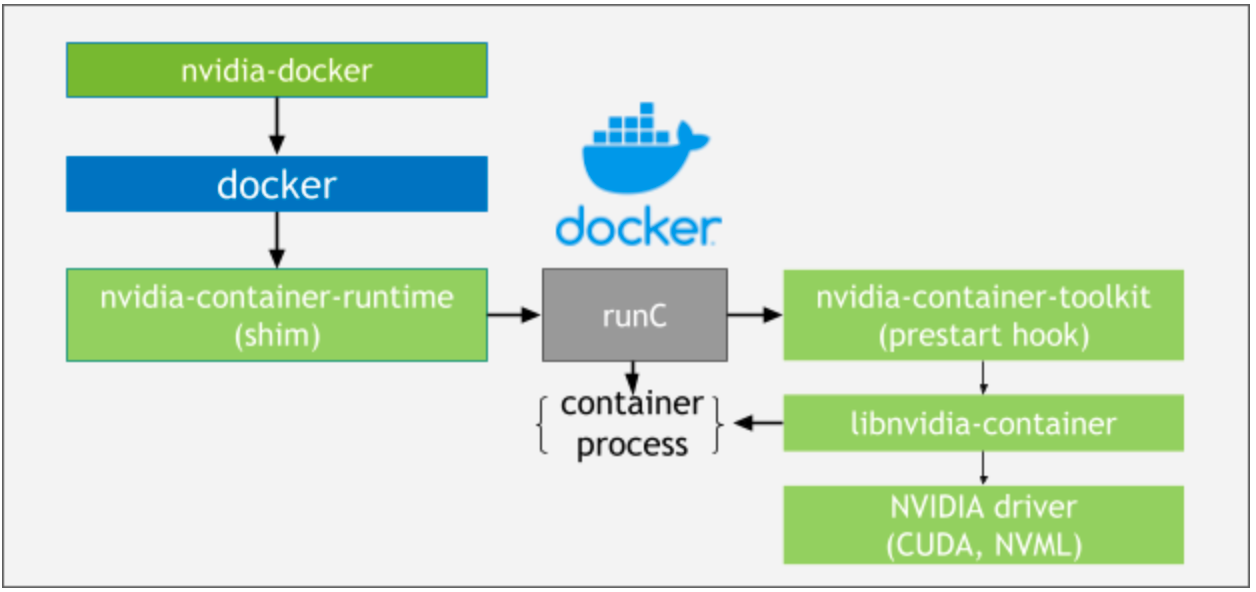
\includegraphics[width=0.9\linewidth]{immagini/Technologies/nvidia-docker-arch-new}
	\caption[Nvidia-docker architecture.]{Nvidia-docker architecture.}
	\label{fig:nvidia-docker-arch-new}
\end{figure}
This toolkit can be an interesting addition for implementing Game Engine graphics modules. However, it is currently not compatible with Docker-compose, which is also an important tool for building distributed system applications.

\section{ETCD}
ETCD is described as a disk-based, distributed and reliable Key-Value Store, which allows the storage of data that can be accessed by a distributed system \cite{site:etcd-desc}. More specifically, ETCD is designed to reliably store infrequently updated data, exposing previous versions of key-value pairs to support inexpensive snapshots of the DB$_G$ and watch history events \cite{site:etcd-data-model}. \\ \\
In order to provide these features, ETCD presents a persistent, multi-version, concurrency-control data model for its key-value storage. This component preserves the previous version of any key-value pair when its value is overwritten with new data. As such, this storage system is described as immutable, since its operations do ot update the structure in-place, but instead generate a new updated structure, where all past versions of the keys are accessible and watchable after modification. \\ \\
In order to guarantee the storage of strongly consistent data, ETCD uses a leader-based consensus protocol called \textit{Raft} for data replication and log execution. The implementation of such algorithm, as well as the rest of ETCD architecture, is developed in the Go programming language, which is particularly fitting for distributed system environments.

\subsection{The Raft Algorithm}
The Raft algorithm is typically adopted in the context of \textit{state machine replication (SMR)} \cite{site:state-machine-replication-wiki}, which is a general method for implementing a fault-tolerant service. This is done by replicating servers (or nodes) and coordinating client interactions with the server replicas. \\
The state machine can be defined as a combination of:
\begin{itemize}
	\item a set of \textit{states};
	\item a set of \textit{inputs};
	\item a set of \textit{outputs};
	\item a transition function, described as: $input \times state \rightarrow state$; 
	\item an output function, described as: $input \times state \rightarrow output$;
	\item a specific \textit{state} called \textit{start};
\end{itemize}
The maximum number of machine replicas that can fail, while still keeping the system operating, is defined by the \textit{crash-fault tolerance}. Moreover, the state machine is required to be \textit{deterministic}, which means that its replicas, starting from the same state and receiving the same input, should return the same output. \\ \\
In this context, a consensus algorithm is required in order to determine and preserve the only authoritative version of the command execution history, in a strongly consistent log.
\begin{figure}[h!]
	\centering
	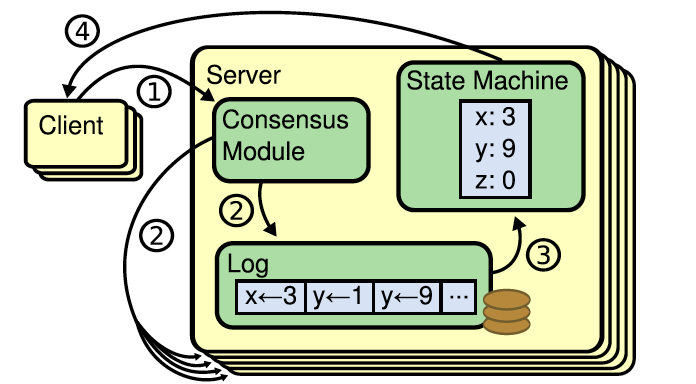
\includegraphics[width=0.7\linewidth]{"immagini/Technologies/image5.png"}
	\caption{Replicated state machine interactions.}
	\label{fig:states}
\end{figure}
\subsubsection{Algorithm overview}
The main goal of the Raft algorithm is to allow distributed nodes to achieve \textit{consensus} on the system state. This means that multiple servers or nodes must agree on some data value that is needed during computation \cite{site:consensus-wiki, site:raft-consensus-algorithm}. This is, generally, a primary objective in the design of fault-tolerant distributed systems. \\ \\
The Raft algorithms defines three main roles, which may be assumed by any node in certain specific situations:
\begin{itemize}
	\item \textit{Follower}: which is a simple node that composes the replicated state machine. This is the default role assigned to nodes when they become part of the \textit{server cluster}, which we define as the subset of nodes that implements the Raft algorithm in a distributed system. Follower nodes may only respond to Candidate and Leader nodes;
	\item \textit{Candidate}: which is a node competing with other Candidate nodes to assume the role of Leader of the distributed system. Nodes may assume this role to request a Leader election, in a situation in which the current Leader node is unresponsive;
	\item \textit{Leader}: which is unique and the only node that interacts with the client. Any request made to Follower nodes is redirected to the Leader node.
\end{itemize}
As previously mentioned, these roles are very important for Raft to be implemented for asymmetric multi-server distributed systems.
\begin{figure}[h]
	\centering
	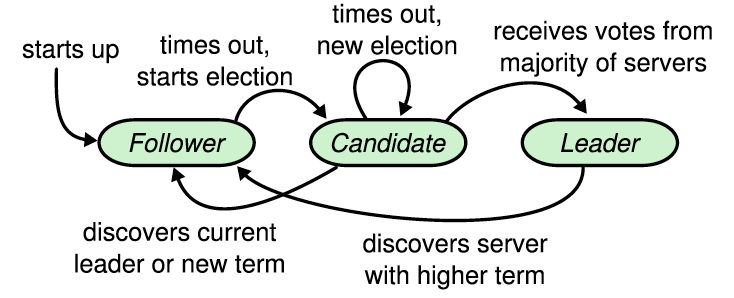
\includegraphics[width=0.7\linewidth]{"immagini/Technologies/image3.png"}
	\caption{Representation of the Raft roles.}
	\label{fig:roles}
\end{figure}
\subsubsection{Time management}
In order to correctly handle server states, the Raft algorithm manages the time by dividing it in \textit{terms} \cite{site:raft-consensus-algorithm}. \\
Working in an asynchronous environment, these terms are not identified by a fixed real-time length. Different servers may observe the transition between terms at different times, while the most significant element of reference is actually the local state of each server. As such, the terms are meant to act as a logical clock, allowing servers to detect obsolete information and stale Leaders, regardless of the asynchronous nature of the system. \\ \\
Each term is uniquely identified by a monotonically increasing integer number called \textit{term number}. This number is stored in each node and attached in node communications. \\
Each term starts with a Leader election, where the Candidates request votes to other server nodes (Followers) in order to obtain a majority consensus:
\begin{itemize}
	\item if a Candidate node manages to obtain the majority of the votes, that Candidate becomes the Leader for the current term;
	\item if no Candidate node manages to obtain the majority of the votes, this situation is called \textit{split vote} and the term will conclude with no elected Leader.
\end{itemize}
As such, a term can only have one single Leader at any time. Moreover, the term number is also a very important indicator for various system tasks, such as:
\begin{itemize}
	\item \textit{term number update}: if a node term number is lower than the one of the other nodes in the cluster, it will be updated at the beginning of a new term. The term numbers used for reference are the ones of the Candidates and the one of the Leader, which usually takes the priority;
	\item \textit{role demotion}: if a Candidate or Leader term number is lower than the other nodes in the cluster, they are demoted to Followers;
	\item \textit{node communication}: the term number of a node is sent as an attachment to each request they make to other nodes. If a request is made with an outdated term number, it is always discarded.
\end{itemize}
This makes the term number a crucial factor in time management, for the Raft algorithm.

\begin{figure}[h]
	\centering
	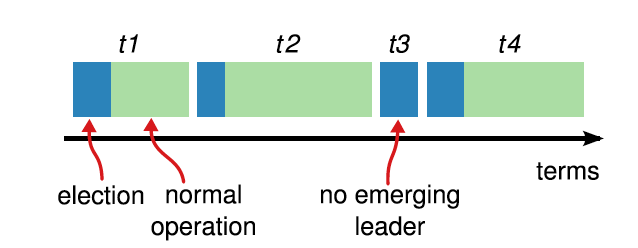
\includegraphics[width=0.7\linewidth]{"immagini/Technologies/image2.png"}
	\caption{Representation of terms (\textit{t\#}).}
	\label{fig:terms}
\end{figure}
\subsubsection{Leader election}
In order to maintain the authority as Leader of the cluster, the node sends periodic messages to the other Follower nodes. These communications are called \textit{heartbeats} \cite{site:raft-consensus-algorithm}. \\ \\
When a Follower node doesn't receive a heartbeat within a given time bound, it assumes the Leader is not active anymore and promotes itself to the role of Candidate. It then votes for itself and requests other nodes to vote for itself, in order to establish a majority. The result of the election can be one of:
\begin{itemize}
	\item the Candidate node receives a vote from the majority of the nodes of the cluster, making it the new Leader. In that moment, the node begins to send heartbeats to notify other nodes of the presence of a new Leader. Candidate nodes receiving the heartbeat will return to the Follower role;
	\item the Candidate node does not manage to get votes from the majority of the nodes of the cluster. In this case, the election ends with no Leader and the node returns to the Follower role;
	\item if the term number of the Candidate node who requested the votes is lower than other Candidate nodes in the cluster, the request is immediately refused and the other nodes keep their Candidate role.
\end{itemize}
This whole process is performed multiple times during the Raft algorithm lifecycle in distributed systems. It ensures that a Leader is always present to serve clients requests and that is condition to do so.
\subsubsection{Log replication}\label{etcd-replication}
Each request made by a client is stored by the Leader in the \textit{logs}, which are then replicated in the other Follower nodes \cite{site:raft-consensus-algorithm}. \\
Generally, a log entry contains the following information:
\begin{itemize}
	\item \textit{command}: which is the instruction specified by the user to be executed;
	\item \textit{index}: which is the number used to identify the position of the entry in the node log, starting from $1$;
	\item \textit{term number}: which is used to ensure the time of a command specific entry.
\end{itemize}
The Leader node requests, through a broadcast, that all the Follower nodes synchronize their logs with its own. The Followers shall reply with an acknowledgment, to confirm the completion of such operation, as the Leader will continue to broadcast synchronization requests until all the other nodes have performed it. \\ \\
A new entry, in this context, is considered \textit{committed} when the majority of the nodes in the cluster has successfully copied it in their logs. At that point, the Leader itself confirms the addition of the entry to its own log, representing the successful outcome of the replication. Following this procedure, it is possible to guarantee that all the previous entry of the log are also committed, otherwise they would not be present inside the log. \\
After an entry has been committed, the Leader carries out the request present in the entry and responds to the client with its result. In this way, the entries are always executed in the same order they are received and confirmed. If two entries in different logs have the same index and term number, it is guaranteed that they contain the same command and that the logs are identical until the specified index. \\ \\
In a situation in which the Leader node crashes, the logs may become inconsistent, since it is the entity responsible for fixing conflicts in the Follower nodes. In this case, the protocol ensures a new Leader is elected, which will look for the last coherent Index in the Followers logs and then overwrite every entry beyond that specific Index with its own. This whole process ensures that the logs of the Followers always match with the Leader and guarantees that the system can provide \textit{Strong Consistency} for the stored data.

\subsubsection{Safety}
In order to maintain \textit{Strong Consistency} of data on a set of server nodes, the Raft algorithm ensures that the Leader is storing all the entries related to previous terms, committed inside its own log. \\
During Leader election, the request for a vote that a Candidate sends to other nodes, also contains some information regarding the log of the Candidate. This information includes the term number of said node, which can be evaluated by the receiver, to immediately discard requests from not updated nodes. \\ \\
In addition to this rule, there are also several other design choices, which help avoid breakage of consensus \cite{site:raft-consensus-algorithm}:
\begin{itemize}
	\item \textit{leader election safety}: there shall be at most one Leader for each term;
	\item \textit{log matching safety}: if multiple logs contains an entry with the same Index and Term, then those logs are guaranteed to be identical, till the given index;
	\item \textit{leader completeness}: the log entries which are committed in a given term shall always appear in the log of the Leader;
	\item \textit{state machine safety}: if a server applied a particular log entry to its state machine, then no other node in the cluster shall apply a different command in its own log;
	\item \textit{leader is append-only}: a Leader node can only add commands at the end of its log. No other data altering operation is allowed;
	\item \textit{follower node crash}: when a Follower node crashes, all the requests sent to the crashed node are ignored. Moreover, the crashed node cannot take part to any Leader election. When the node is restarted, it shall synchronize with the Leader.
\end{itemize}
These characteristics of the Raft algorithm are considered to be sufficient, in order to ensure correct management of operations. Still, the implementation of Strong Consistency is generally expensive in term of computational time, since it requires the system to await for the majority of nodes to synchronize with the Leader, before acknowledging the completion of write operations. \\
As such, it is possible that the performance of this system may not be ideal in contexts where the stored data is changed frequently.

\subsection{Interaction with ETCD}\label{ETCD-interaction}
ETCD allows direct interactions from the client through specific requests, which generally include functionalities \cite{site:etcd-doc} such as:
\begin{itemize}
	\item \textit{write key}: where the client, communicating with any node of the ETCD cluster, instruct the distributed system to write a new key-value or modify an existing key-value. Following the Raft algorithm, if this type of request is sent to a Follower node, it is redirected to the Leader for the actual processing;
	\item \textit{read key}: where the client, communicating with any node of the ETCD cluster, asks for the value of a specific key. According to ETCD configurations, this type of request can be carried out by any ETCD cluster member, since they are constantly updated on the current state of the stored data \cite{site:etcd-faq}.
\end{itemize}
On a more practical level, these requests can be sent either using a dedicated ETCD CLI$_G$ or through ETCD libraries/APIs$_G$ developed in order to allow for interaction also within applications written in different programming languages. In our work, which focuses on code written in C++, the library of choice was \texttt{etcd-cpp-apiv3} \cite{site:etcd-cpp-apiv3}, which is considered to be one of the most updated and reliable ones. \\ \\
Other functionalities \cite{site:etcd-doc} provided by ETCD CLI$_G$ and APIs$_G$ are:
\begin{itemize}
	\item \textit{delete key}: which requests the delete of a specific key-value from the ETCD database;
	\item \textit{watch key}: which is an interesting functionality, that allows clients to subscribe to value updates of specific keys, in order to be notified in real time. This feature is can be particularly helpful when implementing communication through shared memory, since it removes the need for clients to continuously poll the data, in order to verify the presence of changes;
	\item \textit{transactions}: used to perform certain operations when one set of conditions is met or perform other operations when the conditions are not met;
	\item \textit{leases}: mechanism generally used to detect whether a node is alive in the distributed system.
\end{itemize}
All these remote requests and functionalities, which allow the client to communicate with the ETCD system, are carried out using the HTTP protocol. This allows ETCD to leverage all the features provided by such protocol, including \textit{pipelining}: feature that allows the transmission of multiple requests in a single TCP packet, possibly improving the performance of the system. \cite{site:http-pipelining}
\begin{figure}[h!]
	\centering
	\includegraphics[width=0.85\linewidth]{"immagini/Technologies/ETCD cluster"}
	\caption[Example of ETCD cluster with Docker interaction.]{Example of ETCD cluster with Docker interaction.}
	\label{fig:etcd-cluster}
\end{figure}

\subsection{Docker compatibility}
Considering the distributed nature of the ETCD system, it is possible to actually implement ETCD nodes as Docker containers. They can be run both in standalone mode and in cluster mode \cite{site:etcd-docker} with other ETCD containers, communicating using the Docker networking features. \\
Moreover, as shown in figure \ref{fig:etcd-cluster}, different applications running on other Docker containers can connect and interact with the containerized ETCD system, using language-specific APIs$_G$ or, if installed on the app container, directly the ETCD CLI$_G$.

\subsection{System maintenance}
ETCD clusters and nodes require periodic maintenance to remain reliable. Depending on the needs of the ETCD application, the maintenance can be automated and performed without downtime or significantly degraded performance \cite{site:etcd-maintenance}. \\ \\
The ETCD system, in fact, keeps an exact history of its keyspace, which should be periodically compacted in order to avoid performance degradation and eventual storage space exhaustion. On a more technical level, compacting the keyspace history drops all information about keys superseded prior to a given keyspace revision (version of the key). This operation can be configured to be performed periodically or after a set number of key revisions. \\ \\
This freed space should then become available for additional writes to the keyspace. However, in order to completely free the computational resource of the host, an additional operation called \textit{defragmentation} is required. This operation releases the storage space still being consumed by the internal fragmentation of the backend database, and needs to be issued manually for each ETCD member, so that cluster-wide latency spikes may be avoided. \\ \\
Even if the compaction operation can be performed automatically, maintaining the ETCD system using these tools can be quite expensive, both in computational terms and in practical terms, since the defragmentation can only to be launched manually when needed.

\section{Redis}
Redis is an open source, in-memory data structure store used as database, cache, message broker and streaming engine \cite{site:redis-doc}. Redis provides support for multiple different data structures, such as:
\begin{itemize}
	\item strings;
	\item hashes;
	\item lists;
	\item sets;
	\item sorted sets with range queries;
	\item bitmaps;
	\item hyperloglogs;
	\item geospatial indexes;
	\item streams;
\end{itemize}
which can all be managed inside the key-value storage provided by the system. It is also possible to run atomic operations on these types (e.g. appending to a string, incrementing the value of an hash, push an element to a list), dedicated to the specific characteristics of the targeted data structure. \\
Differently from ETCD, which works mainly by operating on the disk, Redis works with an in-memory dataset, which can optionally be periodically dumped on to the disk in the form of snapshots. \\
The software is written in ANSI C and works with most POSIX systems, without external dependences.

\subsection{Features and configurations}
This system provides many interesting and, sometimes, unique features that can prove useful when managing a distributed system \cite{site:redis-doc}. These include:
\begin{itemize}
	\item \textit{LUA scripting}: used for writing scripts that interact with the keys stored in the database;
	\item \textit{eviction policies}: for managing which data should be deleted in case a set memory limit is reached, in term of resource consumption. These policies usually take into consideration the frequency with which a value is accessed (e.g. Least Frequently Used - LFU) or the last time the value was accessed (e.g. Least Recently Used - LRU);
	\item \textit{transactions}: used for executing multiple commands at the same time, in a serialized manner, or in order to place condition on the execution of specific requests;
	\item \textit{on-disk persistence}: with different levels, which allow the system to work directly in-memory or to periodically snapshot the database on the disk;
	\item \textit{creation of distributed systems}: which are highly available thanks to the Eventual Consistency nature of the Redis system;
	\item \textit{publish/subscribe paradigm}: based on events triggered by multiple type of occurrences, both related to messages (e.g. received, sent) and key values (e.g. changes, deletion, addition);
	\item \textit{client-side caching}: this functionality be configured client-side, in order to decide which information to query from the Redis database and which to manage locally through a cache. This decision is typically tied to the frequency of changes that specific key is subject to (measured through the publish-subscribe mechanism);
	\item \textit{pipelining}: implemented for managing multiple read and write requests with a reduced amount of read/write sys calls to the socket methods. This is particularly useful when dealing with multiple clients performing a large number of requests in the same time interval.
\end{itemize}
Additionally, if required by the context of application, it is also possible to configure \textit{Redis itself as a cache}, making all the stored keys "live" only for a certain period of time, before being deleted.

\pagebreak

\subsection{Replication and synchronization mechanism}
At the base of Redis replication there is a Leader-Follower (Master-Follower) consensus mechanism \cite{site:redis-replication}. Similarly to the Raft algorithm, it allows replica Redis instances to be exact copies of Master instances. \\
Moreover, the replica automatically reconnect to the Master every time the link breaks, and attempt to be an exact copy of it regardless of what happens to the master. On a general level, the Redis mechanism works very similarly to the Raft algorithm implemented in ETCD, with the same roles and principles at its basis (e.g. Leader election, log replication). \\ \\
There are, however, very important differences to consider, which highlight the different approaches of the two systems to data consistency. \\
First of all, Redis replicas (Followers) do not accept write requests in their default configuration, differently from ETCD where these requests are redirected by the Followers to the Leader. This is done in order to prevent multiple members to expose view of the distributed DB$_G$ which is different from the one of the Leader. \\ \\
The second difference is related to the management of members disconnections. In ETCD full snapshots of the database are periodically stored on the disk by the single members, and in case of disconnection they always request full synchronization of the last snapshot to the Leader. In Redis, on the other hand, snapshots of the DB$_G$ are not stored on the disk, in the default non-persistence configuration. As such, when disconnections happen the member request just partial synchronization with the current log of the Master, only for the commands lost during the downtime. Full synchronization requires, in fact, the creation of a new complete snapshot of the Master's DB, which is a computationally expensive operation. As such, this process is performed only in cases when partial synchronization is not possible. \\ \\
The third, and most important, difference is related to the management of write requests. In ETCD, as mentioned in section \ref{etcd-replication}, the Leader waits for the write operation to be \textit{commited}, before sending the positive result to the client which requested it. This is an important aspect, which characterizes a system with Strong Consistency of data as a priority. \\
However, in Redis, this is considered to be time-inefficient. As such, when managing write requests, Redis immediately sends a positive result to the Client, as soon as the writing has been completed on the Master's log, without waiting for the replicas synchronization. \\
This might become problematic in situations where the Master node crashes before the synchronization with the replicas is complete, since the Followers will not have inside their logs the write requests that has been declared completed to the Client. As such, this system cannot be defined as Strongly Consistent. However, considering that the replicas will still, in the end, contain the same data inside their databases, this system provides Eventual Consistency of the stored data. \\ \\
In general, we can assert that the main difference between the ETCD and Redis systems management of data is in their approach to consistency. ETCD focuses heavily on Strong Consistency, even at the expense of system performance. Whereas, Redis focuses on providing good performance in standard situations, while accepting the possibility of temporarily losing consistency in some edge cases (Eventual Consistency).

\begin{figure}
	\centering
	\includegraphics[width=0.85\linewidth]{"immagini/Technologies/Redis cluster"}
	\caption[Representation of Redis cluster replication with Docker.]{Representation of Redis cluster replication with Docker.}
	\label{fig:redis-cluster}
\end{figure}

\subsection{Interaction with Redis}
Similarly to ETCD, Redis also provides CLI$_G$ commands (\texttt{redis-cli}) that can be used to interact with the Redis instance from command line. \\
Moreover, regarding the possibility to interact with the Redis instance from applications written in specific programming languages (e.g. C++), Redis provides a list of APIs$_G$ that can be used for this purpose \cite{site:redis-clients}. \\
In particular, for our project, the most fitting option is the \texttt{redis-plus-plus} C++ API$_G$ \cite{site:redis-plus-plus}, which is fairly more complex than the previously mentioned ETCD alternative, but provides a large amount of interesting functionalities. \\ \\
In term of key-value interactions, the features provided include all the ones mentioned in section \ref{ETCD-interaction} for ETCD, with the addition of:
\begin{itemize}
	\item \textit{pipelined requests}: to be configured directly in-code, by inserting requests into the pipeline structure and then call a dedicated method for their execution;
	\item \textit{publish-subscribe mechanism}: which is socket-based and allows the notification of clients through specific messages.
\end{itemize}

\subsection{Docker compatibility}
Considering the distributed nature of the Redis system, it is possible to actually implement Redis nodes as Docker containers. They can be run both in standalone mode and in cluster mode \cite{site:redis-docker-guide} with other Redis containers, communicating using the Docker networking features. \\
Moreover, as we can see in figure \ref{fig:redis-cluster}, different applications running on other Docker containers can connect and interact with the containerized Redis system, using language-specific APIs$_G$ or, if installed on the app container, directly the Redis CLI$_G$.

%\section{System V IPC}
%\intro{General description of System V IPC, its features and aspects considered during our work.}

%\section{X Window System (X11)}
%\intro{General description of X11, its features and general use case scenario.}

%\section{ZeroMQ}
%\intro{General description of ZeroMQ and its features.}
             % Kick-Off
% !TEX encoding = UTF-8
% !TEX TS-program = pdflatex
% !TEX root = ../tesi.tex

%**************************************************************
\chapter{Analisi dei requisiti}
\label{cap:analisi-requisiti}
%**************************************************************

\intro{Breve introduzione al capitolo}\\

\section{Casi d'uso}

Per lo studio dei casi di utilizzo del prodotto sono stati creati dei diagrammi.
I diagrammi dei casi d'uso (in inglese \emph{Use Case Diagram}) sono diagrammi di tipo \gls{uml} dedicati alla descrizione delle funzioni o servizi offerti da un sistema, così come sono percepiti e utilizzati dagli attori che interagiscono col sistema stesso.
Essendo il progetto finalizzato alla creazione di un tool per l'automazione di un processo, le interazioni da parte dell'utilizzatore devono essere ovviamente ridotte allo stretto necessario. Per questo motivo i diagrammi d'uso risultano semplici e in numero ridotto.

\begin{figure}[!h] 
    \centering 
    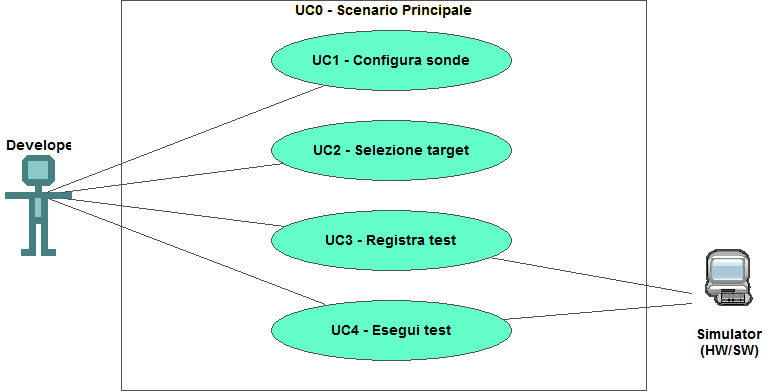
\includegraphics[width=0.9\columnwidth]{usecase/scenario-principale} 
    \caption{Use Case - UC0: Scenario principale}
\end{figure}

\begin{usecase}{0}{Scenario principale}
\usecaseactors{Sviluppatore applicativi}
\usecasepre{Lo sviluppatore è entrato nel plug-in di simulazione all'interno dell'IDE}
\usecasedesc{La finestra di simulazione mette a disposizione i comandi per configurare, registrare o eseguire un test}
\usecasepost{Il sistema è pronto per permettere una nuova interazione}
\label{uc:scenario-principale}
\end{usecase}

\section{Tracciamento dei requisiti}

Da un'attenta analisi dei requisiti e degli use case effettuata sul progetto è stata stilata la tabella che traccia i requisiti in rapporto agli use case.\\
Sono stati individuati diversi tipi di requisiti e si è quindi fatto utilizzo di un codice identificativo per distinguerli.\\
Il codice dei requisiti è così strutturato R(F/Q/V)(N/D/O) dove:
\begin{enumerate}
	\item[R =] requisito
    \item[F =] funzionale
    \item[Q =] qualitativo
    \item[V =] di vincolo
    \item[N =] obbligatorio (necessario)
    \item[D =] desiderabile
    \item[Z =] opzionale
\end{enumerate}
Nelle tabelle \ref{tab:requisiti-funzionali}, \ref{tab:requisiti-qualitativi} e \ref{tab:requisiti-vincolo} sono riassunti i requisiti e il loro tracciamento con gli use case delineati in fase di analisi.

\newpage

\begin{table}%
\caption{Tabella del tracciamento dei requisti funzionali}
\label{tab:requisiti-funzionali}
\begin{tabularx}{\textwidth}{lXl}
\hline\hline
\textbf{Requisito} & \textbf{Descrizione} & \textbf{Use Case}\\
\hline
RFN-1     & L'interfaccia permette di configurare il tipo di sonde del test & UC1 \\
\hline
\end{tabularx}
\end{table}%

\begin{table}%
\caption{Tabella del tracciamento dei requisiti qualitativi}
\label{tab:requisiti-qualitativi}
\begin{tabularx}{\textwidth}{lXl}
\hline\hline
\textbf{Requisito} & \textbf{Descrizione} & \textbf{Use Case}\\
\hline
RQD-1    & Le prestazioni del simulatore hardware deve garantire la giusta esecuzione dei test e non la generazione di falsi negativi & - \\
\hline
\end{tabularx}
\end{table}%

\begin{table}%
\caption{Tabella del tracciamento dei requisiti di vincolo}
\label{tab:requisiti-vincolo}
\begin{tabularx}{\textwidth}{lXl}
\hline\hline
\textbf{Requisito} & \textbf{Descrizione} & \textbf{Use Case}\\
\hline
RVO-1    & La libreria per l'esecuzione dei test automatici deve essere riutilizzabile & - \\
\hline
\end{tabularx}
\end{table}%             % Concept Preview
% !TEX encoding = UTF-8
% !TEX TS-program = pdflatex
% !TEX root = ../tesi.tex
%**************************************************************
\chapter{Software development}
\label{cap:development}
%**************************************************************

\intro{This chapter discusses the development done on the TORCS codebase, including the evaluation of multiple projects as possible starting point. The discussion includes the \textbf{containerization} of the main TORCS system components, the introduction of \textbf{additional software} and the development of \textbf{new components}.}\\

\section{Codebase definition}
Before beginning the work on the TORCS codebase, we performed an exploration and analysis of some TORCS related projects. In the following sections we discuss the two most relevant proposals we identified.

\subsection{Patched TORCS 1.3.7}\label{patched-torcs}
This project takes inspiration from the previously mentioned SCR architecture, introducing significant enhancements to the original TORCS software. It presents a codebase which is mostly congruent with the original 1.3.7 (latest) version of TORCS \cite{site:patched-torcs}. 
\subsubsection{Original TORCS 1.3.7}
The original codebase, in particular, includes the following high-level directories:
\begin{itemize}
	\item \textit{data}: containing useful data information about car models, tracks and UI$_G$ elements;
	\item \textit{doc}: containing general documentation related to the project functionalities and structure;
	\item \textit{src}: containing the actual source code for the software, with its libraries and modules.
\end{itemize}
Inside the source code directory, we can find multiple lower-level directories related to the Game Engine modules and libraries, such as:
\begin{itemize}
	\item \textit{libs}: containing multiple TORCS utility libraries, as well as core components such as the \texttt{raceengineclient}, which is used to manage the main loop of the application;
	\item \textit{drivers}: containing various AI$_G$ implementations for handling robots (cars) behaviour. It also contains an "human" driver, with code related to user manual control of a car;
	\item \textit{graphic}: containing code related to \texttt{ssgraph}, with elements to manage special effects, sound and general rendering of graphical elements;
	\item \textit{simu}: containing code related to the management of the two possible types of simulation provided. This includes physic elements (e.g. collisions), but also data about the actuators functionalities used to drive the car (as described in section \ref{sensors-actuators});
	\item \textit{track}: containing code for managing the build, structure and status of the racing tracks. 
\end{itemize}
The two main enhancements provided by this project are: an implementation of the \textit{SCR-server} for managing the client-server communication with the robots, and a patch which allows to send the game image to another application using \textit{IPC shared memory}.

\subsubsection{SCR-server}
The SCR-server implementation is composed of multiple files related to the management of the robot's sensors (e.g. mathematical computation of the readings) and a single file dedicated to define the actual behaviour of the server in the context of state-action communication. In particular, the server provides three main functions to: \textit{initialize} a new race, \textit{drive} during the race and \textit{end} the current race. In order to start a new race, the component operates as follows:
\begin{enumerate}
	\item binds a listen socket to a specific port (e.g. 3001);
	\item waits for clients to connect and identifies them;
	\item initializes the sensors for sending information to the client robots.
\end{enumerate}
The function dedicated to driving the robot is more complex, since in manages a communication loop with the various remote drivers, operating as follows:
\begin{enumerate}
	\item sends an identification message to each client using a socket;
	\item updates the related sensors;
	\item builds a string representing the current game state;
	\item sends the state string to the remote clients;
	\item waits (with a timeout) for a response action from the clients;
	\item sets the control commands to the input action received and computes the next game state;
	\item if no input is received and the timeout is reached, the old commands are used instead, to compute the next game state.
\end{enumerate}
This configuration is particularly interesting for the purpose of our work, since it manages to successfully decouple the driver component from the main TORCS executable and also to implement the communication of the game state without the usage of pointers.

\subsubsection{screenpipe component}
As previously mentioned, this project tries to introduce the possibility of remotely streaming the game image to a different application, using a dedicated patch. This patch introduces two components, one for obtaining the game image data and serialize it (\texttt{IPC\_command.cpp}), and one for remotely receiving and processing such data (\texttt{screenpipe\_client.py}). As suggested by the files extensions, the components are written in C++ ad Python respectively. \\ \\
In particular, the software and libraries used to accomplish such task are the following ones:
\begin{itemize}
	\item \textit{ZeroMQ}: which is a messaging library for distributed systems, used in both screenpipes's streaming components implement a socket-based communication. The peculiarity of the socket objects created using this library is the possibility to handle asynchronous messages;
	\item \textit{OpenCV}: used as a real time artificial vision library, it is able to both obtain the image from the main game display (in the form of data) and also to reconstruct this same game image, based on the data transferred using the socket-based communication;
	\item \textit{System V IPC}: which is a package able to provide shared memory between multiple processes on the same system, allowing them to share parts of their virtual space. In this context of application, it is used to allow the game image obtained from the main TORCS executable to be transferred to the local streaming component, run in a different executable;
	\item \textit{Google protocol buffers}: used as a data format for serialization and exchange of streaming-related data.
\end{itemize}
While providing an reasonable starting point for implementing streaming communication, this configuration is incomplete in the version provided by the original project. As such, in our work, we elaborate more on this proposal, actually implementing a distributed version of game image streaming.

\begin{figure}
	\centering
	\includegraphics[width=0.8\linewidth]{"immagini/Software development/patched-torcs-architecture"}
	\caption[Proposed streaming architecture]{Proposed streaming architecture.}
	\label{fig:patched-torcs-architecture}
\end{figure}


\subsection{PyTorcs-docker}
This projects is a further development, conducted starting from the previously discusses Patched TORCS 1.3.7 project \cite{site:pytorcs}. More specifically, this proposal aims to implement a Python wrapper of the TORCS software, instantiable on Docker and using System V IPC to manage the game state. \\ \\
In order to efficiently run graphic components on Docker containers, this project proposes the usage of \textit{NVIDIA Docker containers}, which have the peculiar characteristic of being GPU accelerated. They are, however, not simple to implement on any system, since they require access to the GPU hardware. Moreover, as of now, they are not compatible with \textit{docker-compose}, which is also an interesting tool for implementing systems composed of multiple Docker containers, like in our work. \\ \\
Similarly to the SCR project, this proposal presents an architecture where the driver is decoupled from the main TORCS executable. However, the PyTorcs architecture also manages to instantiate the executable into a dedicated Docker container, thus taking a step further in the same direction of our work. \\ \\
\begin{figure}
	\centering
	\includegraphics[width=0.9\linewidth]{"immagini/Software development/PyTorcs architecture"}
	\caption[Representation of the PyTorcs architecture.]{Representation of the PyTorcs architecture.}
	\label{fig:pytorcs-architecture}
\end{figure}
As we can see in figure \ref{fig:pytorcs-architecture}, in order to share with the clients the information of the Render engine, the system makes use of \textit{System V IPC} shared memory in a read-only manner (attach-detach, no semaphores). \\ 
Using the \textit{SnakeOil3} library, developed for interfacing with TORCS using server extensions, this architecture is able to setup an UPD connection on port 3001 to the SCR-server and perform a constant state-action communication.

\subsection{Codebase evaluation}
The PyTorcs-docker project can be considered an evolution of the Patched TORCS 1.3.7 project, with some interesting developments that make use of approaches similar to what we intend to accomplish in our work (e.g. decoupling of modules, usage of Docker). \\
There are, however, some important aspects of this project that discourage its choice as a starting point for our work:
\begin{itemize}
	\item introducing a Python wrapper on top of the original TORCS architecture can be problematic for modularization operations, since it could introduce an additional level of complexity when trying to translate the original Game Engine functionalities to a containerized virtual environment;
	\item the usage of System V IPC shared memory and sockets for game state/image is not necessarily the ideal approach in a distributed virtual environment with multiple containers;
	\item the implementation of NVIDIA Docker containers conflicts with the docker-compose tool, which is particularly interesting for the purpose of our work;
	\item this project removed multiple TORCS core functionalities (e.g. main menu) for the sake of simplicity. This can limit the scope of our project, which aims to modularize and containerize the TORCS Game Engine as a complete software, with all its single components.
\end{itemize} 
As such, considering the interesting SCR approach to TORCS drivers decoupling, the final decision is to reference the Patched TORCS 1.3.7 codebase as a starting point for our project development.

\section{Containerization of TORCS}
Starting the development from the Patched TORCS 1.3.7 codebase, while the driver module is already decoupled from the main executable, no Docker image is included in the proposed architecture. \\
As such, we develop a new Docker image for the TORCS executable, with a dedicated Dockerfile that can be referenced to build a TORCS Docker container using the command \texttt{docker build}. This Docker image is based on the code provided at the project repository, which we call \href{https://github.com/DrSgre/TORCS_multi_docker}{"TORCS\_multi\_docker"}. \\ \\
The Dockerfile alone, however, is not able to directly import environment variables during the launch of the container. In order to circumvent this limitation, we introduce the \texttt{docker-compose} tool mentioned in section \ref{docker-compose}, which also allows us to run multiple containers at the same time and set cross-container configurations. \\ \\
The possibility to import custom environment variables into the application container is particularly important for the implementation of \textit{X11 (X Window System)}. This architecture-independent system can be used for remote graphical user interfaces and input device capabilities, which are both paramount features required by a virtual container running an interactable video game. More specifically, launching the TORCS Docker container will make use of the local display in order to render the video game image for the user, provided that the required permissions have been granted using the command: \texttt{sudo xhost local:root}. \\ \\
As previously mentioned, in order to make use of the SCR architecture we require a different executable for the client running the driver module. Additionally, the client must be run on an environment that is separated from the main executable. As such, we develop a Docker image dedicated to this SCR client, referencing the code provided by the SCR project for the \href{https://sourceforge.net/projects/cig/files/SCR\%20Championship/Client\%20C\%2B\%2B/}{C++ Client}. \\ \\
Different Docker containers, however, cannot by default communicate with each other, as they are completely separate virtual environments. As such, using \texttt{docker-compose}, we setup a \textit{Docker network}, which creates a bridge between the connected containers, allowing them to exchange data. \\ \\
Finally, the Distributed TORCS architecture presented in figure \ref{fig:development-1} is able to launch the TORCS software application, render its game image on the local display and allow a second container to connect to a "quick race" instance of TORCS.
\begin{figure}[h!]
	\centering
	\includegraphics[width=0.8\linewidth]{"immagini/Software development/Development-1"}
	\caption[Distributed TORCS architecture - phase 1.]{Distributed TORCS architecture - phase 1.}
	\label{fig:development-1}
\end{figure}
 

\section{Distributed databases implementation}
In order to allow the Game Engine modules located in different containers to communicate with each other, a dedicated mean of communication is required. In the implementation proposed by the Patched TORCS 1.3.7 project, the main TORCS executable and the SCR client communicate through a socket-based connection. This is a reasonable choice for simple action-state exchanges, however when multiple modules are accessing and modifying the same shared game state this approach might not be ideal. Inconsistency in the data read by different modules can, in fact, impact the video game functionalities. As such, we decide to implement data communication between the modules using a \textit{shared storage distributed database}. In this context, we evaluate two different solutions, considered to both to be fitting for the purpose of our work, namely: \textit{ETCD} and \textit{Redis}. \\ \\
Both solutions are provided with Docker images (\href{https://hub.docker.com/r/bitnami/etcd}{ETCD image} and \href{https://hub.docker.com/_/redis}{Redis image}) that can be freely implemented into applications, as such the Docker integration is simple and straightforward, provided that said images are configured to be connected to the same Docker network as the other containers. \\ \\
Nonetheless, in order to interact with the distributed databases instances from the TORCS application, we also require APIs$_G$ and libraries dedicated to such purpose. As such, we decide to compile and link into TORCS both: \href{https://github.com/etcd-cpp-apiv3/etcd-cpp-apiv3}{etcd-cpp-apiv3} and \href{https://github.com/sewenew/redis-plus-plus}{redis-plus-plus}. In order to separate the two distributed databases implementations, we have two different and dedicated TORCS applications in our project repository. \\ \\
The results of initial experiments exposed some performance issues with ETCD, mostly caused by the local storage of the history of all the keys that have been changed during execution, alongside multiple expensive DB$_G$ snapshots. As such, we have applied some changes to the original ETCD application, in order to remove said expensive operations and correct some memory management issues arisen in our application context. The new ETCD Docker image referenced in the project is stored in our repository.

\begin{figure}[h!]
	\centering
	\includegraphics[width=0.8\linewidth]{"immagini/Software development/Development-2"}
	\caption[Distributed TORCS architecture - phase 2.]{Distributed TORCS architecture - phase 2.}
	\label{fig:development-2}
\end{figure}

\subsection{OrbitDB}
An additional distributed DB$_G$ we considered for implementation is OrbitDB \cite{site:orbitdb}. This system is a decentralized database that uses the InterPlanetary File System (IPFS) as its storage layer. It is designed to be a lightweight distributed database, which requires no central authority to operate. \\ \\
OrbitDB stores data in a database structure that is similar to a key-value store or a document store. Each database is associated with a unique address, and data is stored in a series of append-only logs that are replicated across the IPFS network. This allows multiple users to access and modify the database concurrently, without the need for a central server. \\ \\
OrbitDB is implemented in JavaScript and designed to be integrated into applications developed using this language (either using Node.js or native). This was considered to be strong limitation, in our context of application, since TORCS is strictly developed in C++, with no way to interact with such system. \\ \\
As such, this solution was discarded, in favour of ETCD and Redis distributed databases.

\subsection{Distributed database clusters}\label{ddb-clusters}
The benefits of Redis Eventual Consistency mechanism, when compared with ETCD Strong Consistency mechanism, are not quite evident in a stand-alone configuration of these distributed databases. The lack of node replicas, in fact, prevents the need for replication operations, which generally slow down the performance of Strong Consistency mechanisms. \\
As such, since this core difference in functionality is not present, and the two systems end up working in a similar manner. \\ \\
In order to more clearly highlight the benefits of the Redis distributed database, we implemented a 3-members cluster version of both Redis and ETCD, integrating it with our TORCS distributed architecture.

\begin{figure}[h!]
	\centering
	\includegraphics[width=0.8\linewidth]{"immagini/Software development/ETCD cluster"}
	\caption[ETCD 3-members cluster configuration.]{ETCD 3-members cluster configuration.}
	\label{fig:etcd-cluster}
\end{figure}
\begin{figure}[h!]
	\centering
	\includegraphics[width=0.8\linewidth]{"immagini/Software development/Redis cluster"}
	\caption[Redis 3-members cluster configuration.]{Redis 3-members cluster configuration.}
	\label{fig:redis-cluster}
\end{figure}
As we can see in Figure \ref{fig:etcd-cluster}, the requests in the ETCD cluster implementation can be sent to any of the ETCD containers, which directly respond to read requests and redirect write requests to the Leader. The choice of which container to send the request is delegated to the ETCD C++ API$_G$, which uses a Round Robin (RR$_G$) strategy to balance out the workload between the instances. \\
In Figure \ref{fig:redis-cluster}, on the other hand, we see how all the requests are directed towards the Redis Master node, which immediately responds to the client upon completion.

\section{Game image streaming}
As previously mentioned in section \ref{patched-torcs}, another interesting functionality implemented in the Patched TORCS 1.3.7 project is the possibility to remotely stream the game image to another display. \\ \\
This functionality is interesting for testing the performance and capabilities of our means of communication (a.k.a. the distributed databases). As such, we proceed with turning the previously socket-based communication into a data exchange performed using the shared memory provided by ETCD/Redis. In this context, the serialized data of the game image is stored into a specific key of the database, while the remote screenpipe component is notified upon each key change and is able to get such information through a read request. \\ \\
Considering the weight of the data information used to describe a complete game image (multiple MBs), it is to be expected that the storage operation is quite expensive for a distributed database. \\
In fact, while the refactoring operation was successful, the streaming performance of the resulting system are not satisfactory, with a very low display framerate (<1 fps). \\ \\
The reason for this low performance lies in the remote client component responsible for rendering the received image, which is not fit for efficiently perform such task. The component is, in fact, incomplete and developed using Python, which is not the best choice for applications required to process large amounts of data swiftly. Moreover, the sending component also performs unnecessary expensive operations, such as serialization and transfers of data between executables using System V IPC shared memory. \\ \\
As such, we perform a complete refactoring of both streaming components (sender and receiver), developing them in C++ and significantly reducing the amount of elaboration operations. The result of this process is a much more efficient streaming functionality, which, despite exchanging data using a distributed database, is able to provide reasonable performance (about 30 fps). \\ \\
Still, considering the excessively large amount of network communication and bandwidth required to implement such functionality at its full potential, we limit the image streaming framerate to 10 frames-per-second.

\begin{figure}[h!]
	\centering
	\includegraphics[width=0.9\linewidth]{"immagini/Software development/Development-3"}
	\caption[Distributed TORCS architecture - phase 3.]{Distributed TORCS architecture - phase 3.}
	\label{fig:development-3}
\end{figure}

\subsection{ETCD changes for resource management}\label{etcd-evolution}
One of the main problems arisen during the implementation of ETCD is the amount of resources needed for the storage of the history of all keys changed during the system execution. This data is stored into the hard drive and memory of the system where ETCD is run. As such, in situations where changes are frequent and the key history data rapidly increases in volume, the resources available can prove not to be sufficient for handling the system operations. \\ \\
This is particularly evident in our context of execution, where the game image streaming, alongside other functionalities later discussed, cause a constant flux of large-sized requests. \\
As such, we operated some changes to the original ETCD software, by:
\begin{itemize}
	\item removing the functionality which caused the saving and update of WAL$_G$ files, used for snapshotting the database;
	\item instruct ETCD to create a new WAL$_G$ folder at each database startup, restarting the database from a standard empty condition.
\end{itemize}
This was considered to be in line with the needs of our project, considering that long term storage of information was not required in this context. While this change greatly reduced the size of the data stored on the disk, the memory resources were still not managed efficiently enough. As such, we made use of two additional built-in ETCD functionalities: \textit{automatic periodic compaction} and \textit{defragmentation}. \\
Since the ETCD defragmentation can only be requested manually, we set up a custom script to perform it at certain intervals of time. \\ \\
Finally, after noticing a delay between the end of the defragmentation operations and the actual freeing of memory resources, we assumed that the system memory management was actually delegated to the Go Garbage Collector. As such, in order to see an immediate effect on the available resources after a defragmentation, we introduced an additional explicit call to the Go Garbage Collector, at the end of the related function. \\ \\
In the end, we managed to keep the actual DB$_G$ in-memory size within 300 MB, during TORCS execution, which was deemed reasonable to guarantee not to reach resource saturation.

\section{Distributed state-action communication}\label{DDB-SA-communication}
As discussed in the previous section, we managed to verify the possibility of replacing socket-based communication between TORCS system components, with a data exchange carried out through the shared memory of a distributed database. \\
We now proceed with performing a similar replacement operation also in the context of the SCR state-action communication that happens between the TORCS main executable and the remote driver. \\ \\
In this context, as described in section \ref{scr}, the SCR-server broadcasts a string representing the game state to all connected peers, awaits their response action and then processes the new game state based on the responses. This whole communication process can be implemented by writing both the game state string and the response action string on different keys in the distributed database, and have the components continuously check for key changes. \\ \\
The result of this implementation is a new SCR client-server architecture, providing the same remote driving functionalities as the original system, but leveraging the characteristics of a distributed database.
\begin{figure}[h!]
	\centering
	\includegraphics[width=0.9\linewidth]{"immagini/Software development/Development-4"}
	\caption[Distributed TORCS architecture - phase 4.]{Distributed TORCS architecture - phase 4.}
	\label{fig:development-4}
\end{figure}


\section{Music Player library}
Up until this point, in the development process, we focused on containerizing Game Engine modules (e.g. AI$_G$ driver) or introduce new functionalities (e.g. distributed databases, remote streaming). The TORCS software, however, is also composed of multiple libraries which may benefit from containerization. \\
These libraries, which we previously mentioned in section \ref{patched-torcs}, are smaller sized with respect to complete TORCS modules. However, they are still responsible for managing core functionalities of the system (e.g. music). \\ \\
Before beginning the decoupling operations, we perform a preliminary analysis on the quantity of external references and dependencies present in some of the libraries. In fact, as the number of references increases, the complexity of the decoupling operation increases as well, considering the side effects on the external referencing components that must also be adapted. \\ \\
The result of this analysis highlights the \textit{musicplayer} library as a reasonable candidate for containerization. This component is dedicated to managing the enabling and disabling of the music in the game menu, and presents no dependency towards other components, making it quite simple to implement as an independent executable. \\ \\
Considering the basic logic exposed by this component's methods, the implementation was realized based on the original socket-based communication between SCR client and server, where:
\begin{enumerate}
	\item the main TORCS executable is launched and listen for messages from the musicplayer on a specific socket port;
	\item the musicplayer component is launched and sends an identification message on a specific socket port, allowing the TORCS executable to identify it and proceed;
	\item the musicplayer then processes any requests for enabling/disabling the menu music, coming from the TORCS executable on the same socket used for identification.
\end{enumerate}
Using this configuration is possible to implement the same original functionalities of the TORCS musicplayer library, as a distributed component.

\begin{figure}[h!]
	\centering
	\includegraphics[width=0.95\linewidth]{"immagini/Software development/Development-5"}
	\caption[Distributed TORCS architecture - phase 5.]{Distributed TORCS architecture - phase 5.}
	\label{fig:development-5}
\end{figure}


\section{State Manager Middleware}\label{state-manager-middleware}
One of the main goals of our development is to be able to effectively distributed information about the TORCS game state among its different decoupled components. However, during our experiments, which we will discuss in the following chapters, we identified a problem in implementing this game state distribution with the same approach as in other development phases (e.g. game image streaming, state-action communication). \\ \\
In previous contexts the processing time required by the distributed databases to elaborate the requests was considered to be reasonable, with a low impact on the system performance. However, this is not the case in the context of TORCS internal game state management, where certain system components (e.g. graphic module, simulation module) present the requirement for rapid access to such data. In fact, the original implementation with C++ pointers, while centralized, is designed to allow for efficient game state data access, even between different system components. \\ \\
In order to both allow for distribution of game state data and prevent significant impact on the system performance, we consider a different approach. \\
We develop a new component, dedicated to managing the storage of the TORCS game state into the distributed database with a set update frequency, independent from the original game loop. This component is also meant to be able to distinguish the nature of the specific game state fields to be stored, depending on the inconsistency tolerance of the user and the frequency of specific values changes, managing the storage operations accordingly. \\ \\
The final goal is to have a background-running component, which is able to independently store or update the current game state, and to provide a reasonable degree of synchronization between multiple distributed TORCS Game Engine states.

\subsection{Technical choices}
This component, which we will call \textit{State Manager middleware}, is run as a different thread, detached from the main TORCS executable, but running in its same environment (Docker container). \\
It makes use of \texttt{etcd-cpp-apiv3} (or \texttt{redis-plus-plus}) to be able to connect to the distributed database container, and perform read/write operations. \\
Moreover, it also includes the \texttt{chrono} and \texttt{thread} libraries, in order to introduce thread sleep lasting less than a second. \\ \\
The update frequency has been set to 100 ms, considering the balance between inconsistency tolerance and the impact on the distributed database performance of frequent requests. Additional tests, with different frequency levels, can be conducted to find the best fitting value for specific system implementations. \\ \\
The component is initialized through its \textit{StartStateManager} method, which is called during the instantiation of a dedicated thread at the start of a new race. This is done in order to allow for background execution, without influencing the TORCS system performance. \\ \\
We also distinguish between \textit{static game state fields}, which are variables that compose the game state that are not updated after a race has been started, and \textit{dynamic game state fields}, which are variable of the game state that are frequently updated during race execution.

\begin{figure}
	\centering
	\includegraphics[width=0.9\linewidth]{"immagini/Software development/Game state manager"}
	\caption[State Manager middleware architecture.]{State Manager middleware architecture.}
	\label{fig:game-state-manager}
\end{figure}

\subsection{Component methods}
The State Manager middleware provides three methods:
\begin{itemize}
	\item \textit{StartStateManager}: accessible from other modules and taking \texttt{tRmInfo} (full game state data) as input parameter, this method performs the initialization of the \texttt{statemanager} component and its update loop;
	\item \textit{SaveState}: only accessible inside the \texttt{statemanager} component and taking the current game state (\texttt{tSituation}) as input parameter, this method performs the storage on the distributed DB$_G$ of the relevant game state fields and car state fields (for all cars);
	\item \textit{LoadState}: only accessible inside the \texttt{statemanager} component and taking \texttt{tRmInfo} as input parameter, this method reads from the distributed DB$_G$ the relevant game state fields and car state fields (for all cars), updating the local state accordingly.
\end{itemize}
We can now elaborate more on each method's elaboration logic.

\subsubsection{StartStateManager}
This method operates with the following logic:
\begin{enumerate}
	\item it checks whether a race is running by verifying if the \texttt{/state/currentTime} key is set in the distributed DB;
	\begin{enumerate}
		\item if it is, the following static game state fields are read from the distributed DB and set in the local game state:
		\begin{itemize}
			\item \texttt{/state/raceType}
			\item \texttt{/state/totLaps}
			\item \texttt{/state/ncars}
			\item \texttt{/state/maxDammage}
		\end{itemize}
		\item otherwise, the following static game state fields are written into the distributed DB:
		\begin{itemize}
			\item \texttt{/state/raceType}
			\item \texttt{/state/totLaps}
			\item \texttt{/state/ncars}
			\item \texttt{/state/maxDammage}
		\end{itemize}
		The following dynamic game state fields are written into the distributed DB, to allow for later comparisons:
		\begin{itemize}
			\item \texttt{/state/deltaTime}
			\item \texttt{/state/currentTime}
			\item \texttt{/state/raceState}
		\end{itemize}
		The following dynamic car state fields are written into the distributed DB, for each car \textit{"i"} to allow for later comparisons:
		\begin{itemize}
			\item \texttt{/carstate/car[i]/pos\_toStart}
			\item \texttt{/carstate/car[i]/pos\_toMiddle}
			\item \texttt{/carstate/car[i]/pos\_toRight}
			\item \texttt{/carstate/car[i]/pos\_toLeft}
			\item \texttt{/carstate/car[i]/seg\_id}
			\item \texttt{/carstate/car[i]/pos\_X}
			\item \texttt{/carstate/car[i]/pos\_Y}
			\item \texttt{/carstate/car[i]/pos\_Z}
			\item \texttt{/carstate/car[i]/pos\_AX}
			\item \texttt{/carstate/car[i]/pos\_AY}
			\item \texttt{/carstate/car[i]/pos\_AZ}
		\end{itemize}
	\end{enumerate}
	\item the game state update loop is started, performing a cycle each 100 ms;
	\item if the race is paused, the \texttt{statemanager} waits without performing requests. Otherwise, it checks whether the distributed DB$_G$ \texttt{/state/currentTime} is different from the local value;
	\begin{enumerate}
		\item if the remote value is greater than the local one, this means that the local GE$_G$ values are outdated and the \textit{LoadState} method is called;
		\item if the remote value is lower than the local one, this means that the local GE$_G$ is able to provide updated state values to the distributed DB$_G$, so the \textit{SaveState} method is called.
	\end{enumerate}
	\item after the Load/Save operations have been performed, the thread sleeps for 100 ms and then starts a new cycle.
\end{enumerate}
Once the race has ended, all the distributed DB$_G$ keys are removed as a clean up operation.

\subsubsection{StartStateManager}
This method operates with the following logic:
\begin{enumerate}
	\item for each dynamic game state field, the remote value is checked and, if different from the local one, it is updated through a write request;
	\item for each dynamic car state field of each car, the remote value is checked and, if different from the local one, it is updated through a write request;
	\begin{itemize}
		\item the following values are related to the position of the car with respect to the specific track segment:
		\begin{itemize}
			\item \texttt{/carstate/car[i]/pos\_toStart}
			\item \texttt{/carstate/car[i]/pos\_toMiddle}
			\item \texttt{/carstate/car[i]/pos\_toRight}
			\item \texttt{/carstate/car[i]/pos\_toLeft}
			\item \texttt{/carstate/car[i]/seg\_id}
		\end{itemize}
		\item the following values are related to the position of the car with respect to the global position:
		\begin{itemize}
			\item \texttt{/carstate/car[i]/pos\_X}
			\item \texttt{/carstate/car[i]/pos\_Y}
			\item \texttt{/carstate/car[i]/pos\_Z}
			\item \texttt{/carstate/car[i]/pos\_AX}
			\item \texttt{/carstate/car[i]/pos\_AY}
			\item \texttt{/carstate/car[i]/pos\_AZ}
		\end{itemize}
	\end{itemize}
\end{enumerate}

\subsubsection{LoadState}
This method operates with the following logic:
\begin{enumerate}
	\item for each dynamic game state field, the local value is checked and, if different from the one in remote value, it is updated accordingly;
	\item for each dynamic car state field of each car, the local value is checked and, if different from the remote one, it is updated accordingly;
	\begin{itemize}
		\item the following values are related to the position of the car with respect to the specific track segment:
		\begin{itemize}
			\item \texttt{/carstate/car[i]/pos\_toStart}
			\item \texttt{/carstate/car[i]/pos\_toMiddle}
			\item \texttt{/carstate/car[i]/pos\_toRight}
			\item \texttt{/carstate/car[i]/pos\_toLeft}
		\end{itemize}
		\item the value related to segment id (\texttt{seg\_id}) is used to iterate on the double linked list present in the local car state, setting the current track segment depending on the id read from the distributed DB.
		\item the following values are related to the position of the car with respect to the global position:
		\begin{itemize}
			\item \texttt{/carstate/car[i]/pos\_X}
			\item \texttt{/carstate/car[i]/pos\_Y}
			\item \texttt{/carstate/car[i]/pos\_Z}
			\item \texttt{/carstate/car[i]/pos\_AX}
			\item \texttt{/carstate/car[i]/pos\_AY}
			\item \texttt{/carstate/car[i]/pos\_AZ}
		\end{itemize}
	\end{itemize}
	\item in order for the car state updates to be reflected in the game simulation, the \textit{\_reSimItf.config()} method is called.
\end{enumerate}

\subsection{Final remarks}
With the introduction of this component into TORCS, we can see at execution time how if we:
\begin{enumerate}
	\item launch an instance of distributed DB.
	\item run a race in a TORCS executable for a certain amount of time.
	\item pause/stop the race.
	\item launch a race on a second TORCS executable.
\end{enumerate}
The \texttt{statemanager} on the second instance immediately synchronizes with the values stored into the distributed DB$_G$, updating the game time and teleporting the car to the position read from distributed DB$_G$.
With some additional enhancements (e.g. add velocity and acceleration car state fields to distributed DB$_G$), it could be possible to implement a synchronization mechanism able to work in a distributed Game Engine environment.

\begin{figure}
	\centering
	\includegraphics[width=0.95\linewidth]{"immagini/Software development/Development-6"}
	\caption[Distributed TORCS architecture - phase 6.]{Distributed TORCS architecture - phase 6.}
	\label{fig:development-6}
\end{figure}

\subsection{Additional development}\label{state-manager-next}
In order to verify the possibility to implement constant game state distribution, between multiple TORCS instances, we perform some changes to the original State Manager configuration. More specifically, we introduce the following modifications:
\begin{itemize}
	\item we increase the update frequency from 100 ms to 1 ms (sleep time);
	\item we allow only the first TORCS instance launched to write on the distributed database, while the TORCS following instances are allowed only to read from the database;
	\item the read-only TORCS instances do not perform local simulation updates, as their state is updated by the State Manager.
\end{itemize}
We also add new car state fields for the storage operations, including speed-related ones:
\begin{itemize}
	\item \texttt{/carstate/car[i]/vel\_X}
	\item \texttt{/carstate/car[i]/vel\_Y}
	\item \texttt{/carstate/car[i]/vel\_Z}
	\item \texttt{/carstate/car[i]/vel\_AZ}
\end{itemize}
And acceleration-related ones:
\begin{itemize}
	\item \texttt{/carstate/car[i]/acc\_X}
	\item \texttt{/carstate/car[i]/acc\_Y}
	\item \texttt{/carstate/car[i]/acc\_Z}
\end{itemize}
With this configuration, we are able to have multiple distributed instances of TORCS reproducing the in-game situation of the first TORCS instance, without any computation being performed by the game engines themselves. Moreover, the system is able to update the remote state of up to 10 cars in the same race.             % Product Prototype
% !TEX encoding = UTF-8
% !TEX TS-program = pdflatex
% !TEX root = ../tesi.tex
%**************************************************************
\chapter{Experimental methodology}
\label{cap:experimental-methodology}
%**************************************************************

\intro{This chapter discusses the single experiments conducted during the project, providing their \textbf{purpose} and \textbf{expected theoretical outcome. Moreover, this chapter introduces the research methods and design that were used to conduct the studies, both for the \textbf{qualitative} and the \textbf{quantitative} experiments.}}

\section{Qualitative experiments}
\intro{The following sections present qualitative experiments, performed in order to obtain a general idea about the effects on the system of specific development decisions. These experiments can provide general numerical data, which is generally \textbf{not} supported by multiple misurations or graphical representations.}

\subsection{ETCD for SCR state-action communication}
\intro{This section presents the introduction of ETCD for SCR state-action communication, as a replacement for the socket-based original alternative.}
\subsubsection{Purpose \& Expected outcome}
\subsubsection{Methods \& Design}

\subsection{Multi-node ETCD cluster}
\intro{This section presents the introduction of an ETCD cluster of 3 members, verifying the effect this had on the system performance.}
\subsubsection{Purpose \& Expected outcome}
\subsubsection{Methods \& Design}


\section{Quantitative experiments}
\intro{The following sections present quantitative experiments, performed in order to obtain precise and numerical data about specific phenomena, effects on the system performance of specific configurations or correlation between system components. The data provided by these experiments is supported by multiple misurations and graphical representations.}

\subsection{X11 forwarding performance assessment}
\intro{This section presents the test conducted in order to verify whether X11 can be considered a bottleneck and have significant impact on the performance of video streaming between two different PCs.}
\subsubsection{Purpose \& Expected outcome}
\subsubsection{Methods \& Design}

\subsection{Game image streaming solutions}
\intro{This section presents the experiment performed in order to measure the video streaming performance of the system with different configurations.}
\subsubsection{Purpose \& Expected outcome}
\subsubsection{Methods \& Design}

\subsection{Network traffic analysis}
\intro{This section presents the experiment performed in order to measure the amount of data processed in I/O from/towards the network or the disk, alongside measuring the round-trip-time between SCR client and server in the same architecture.}
\subsubsection{Purpose \& Expected outcome}
\subsubsection{Methods \& Design}

\subsection{Network latency impact assessment}
\intro{This section presents the experiment performed in order to measure the performance of TORCS and screenpipe displays, in situations with high or moderate network latency in the ETCD container.}
\subsubsection{Purpose \& Expected outcome}
\subsubsection{Methods \& Design}

\subsection{Distribution of dynamic game state data}
\intro{This section presents the experiment performed in order to measure the system performance when introducing the storage of an increasing number of game state data fields into ETCD, alongside an increasing amount of network latency in the ETCD container.}
\subsubsection{Purpose \& Expected outcome}
\subsubsection{Methods \& Design}

\subsection{Distribution of static game state data}
\intro{This section presents the experiment performed in order to measure the system performance when introducing the storage of different static game state data fields into ETCD.}
	\subsubsection{Purpose \& Expected outcome}
	\subsubsection{Methods \& Design}

\subsection{ETCD in-memory persistence}
\intro{This section presents the experiment performed in order to measure the system performance when storing 3 game state data fields in a situation in which ETCD is writing to memory, instead of the Disk.}
	\subsubsection{Purpose \& Expected outcome}
	\subsubsection{Methods \& Design}


\subsection{Graphics and physics engine correlation}
\intro{This section presents the experiment performed in order to verify and quantify the correlation between the graphic and physics engine of TORCS, by introducing an increasing delay into the simulation module and verifying the impact on the graphics framerate. Moreover, we also compute the theoretical framerate bounds generated by the delays and compare them with the actual measured framerate.}
\subsubsection{Purpose \& Expected outcome}
\subsubsection{Methods \& Design}

\subsection{Graphics and game engine framerate correlation}
\intro{This section presents the experiment performed in order to measure the net operational time and the correlation between the GE framerate and the graphics framerate, in a situation in an increasing delay introduced into the simulation module.}
\subsubsection{Purpose \& Expected outcome}
\subsubsection{Methods \& Design}             % Product Design Freeze e SOP
% !TEX encoding = UTF-8
% !TEX TS-program = pdflatex
% !TEX root = ../tesi.tex

%**************************************************************
\chapter{Conclusioni}
\label{cap:conclusioni}
%**************************************************************

%**************************************************************
\section{Consuntivo finale}

%**************************************************************
\section{Raggiungimento degli obiettivi}

%**************************************************************
\section{Conoscenze acquisite}

%**************************************************************
\section{Valutazione personale}
             % Conclusioni
% !TEX encoding = UTF-8
% !TEX TS-program = pdflatex
% !TEX root = ../tesi.tex

%**************************************************************
\chapter{Conclusion}
\label{cap:conclusion}
\intro{This chapter provides a final discussion about the outcome of the whole research effort, considering also the \textbf{limitations} of the study design and findings, and the \textbf{recommandations for future research}.}

\section{Final assessment}
In this work, we investigated the feasibility of containerizing Legacy Game Engine modules and having them communicate with each other, with the purpose of implementing a Distributed Game Engine architecture. Our results show that it is indeed possible to containerize these modules and have them communicate with each other using various inter-container communication techniques. \\ \\
Moreover, we also explored the use of distributed databases as a solution for allowing consistent, but not necessarily quick, data communication between the Game Engine modules. We found that distributed databases can be a viable option for ensuring data consistency between modules, although their performance may not always meet the high-speed requirements of some gaming applications, such as TORCS. \\ \\
To this end, we compared the performance of Redis and ETCD in the context of a distributed version of TORCS. We found that Redis generally provided better framerate compared to ETCD, both in their standalone and 3-member cluster versions. This was evident in the various configurations that we tested, with Redis consistently delivering higher framerate than ETCD, in context where no latency is present. \\
Still, when network latency is introduced, ETCD's implementation of HTTP$_G$ pipelining may provide interesting benefits to mitigate the effect of delays on the single packets, especially in the stand-alone version of the systems, where their difference is not particularly pronounced. \\ \\
In the cluster versions of the systems, the difference in framerate between Redis and ETCD was particularly pronounced. Thanks to its Eventual Consistency mechanism, Redis was able to achieve significantly higher framerate than ETCD, indicating its superior performance in this setting. \\ \\
Overall, our results suggest that Redis is a more suitable choice for distributed applications that require high responsiveness, such as a distributed version of TORCS. On the other hand, ETCD may be more suitable for applications that require strong consistency and support for distributed transactions, but may not be as well-suited for high-performance applications. \\ \\
Working on an alternative solution, we implemented a State Manager middleware as a means of storing and distributing the state of a distributed version of TORCS. Our results showed that the State Manager was able to provide state storage and distribution without significantly impacting the performance of the system and with a generally moderate state inconsistency, in its Redis-based implementation. \\
Our experimental results demonstrated that the State Manager was able to provide fast and reliable state storage and distribution, with minimal impact on the framerate of the distributed version of TORCS. We also found that the State Manager was able to scale well with increasing numbers of cars, showing good performance even if with some graphics glitches. \\ \\
We also found that network latency has a noticeable impact on the performance of the distributed version of TORCS, leading to a significant degradation in framerate and a less enjoyable gameplay experience. This highlights the challenges of using distributed databases in these types of high-performance and latency-sensitive systems. \\
Despite the use of distributed databases optimized for fast and reliable data storage and retrieval, we found that they did not provide good performance when network latency was introduced. This suggests that more advanced techniques may be needed to effectively handle the high responsiveness requirements of TORCS in a distributed setting.

\section{Limitations}
While the tests conducted in this work were able to provide interesting insights into the performance of a TORCS distributed system based on shared storage, it is important to note that they were conducted in a local Docker environment, rather than a real-world Cloud$_G$ Computing scenario. This means that the results may not necessarily generalize to a production setting, where the system would be deployed on a Cloud$_G$ platform such as Amazon Web Services, Microsoft Azure or Kubernetes. \\ \\
A local Docker environment does not necessarily simulate the network latency and bandwidth constraints that are commonly encountered in a Cloud$_G$ environment. This can lead to differences in performance and resource utilization compared to a real-world context. \\ \\
One additional limitation is that only a few of the TORCS modules and libraries were containerized and incorporated into the final architecture. This means that this distributed version of TORCS is currently not complete, and only serves as a prototype for evaluating the feasibility of this approach. \\ \\
Finally, another limitation is that the State Manager middleware is limited in the amount of game state related data that it can store on the distributed database. The TORCS game state consists of a large amount of data, including information about the track, the cars, and their positions and velocities. In order to maintain a reasonable level of performance, the State Manager can only store a subset of this data on the distributed database. \\ \\
This means that the State Manager is not able to store the full game state at any given time, and some information may be lost or not accurately represented. This could potentially impact the accuracy and representation of the game, as well as generate graphics glitches in the distributed TORCS instances. \\ \\
Despite these limitations, this distributed version of TORCS and the related State Manager middleware developed during this project represent a significant step forward in the development of Distributed Game Engines.

\section{Recommandations for future research}
Considering the limitations we discussed in the previous section, there are multiple areas where future research can be conducted in order to provide interesting additional development. \\ \\
For instance, further work could be done to fully decompose the TORCS system architecture and address other aspects such as security and usability. Multiple additional libraries and modules of the original architecture may require considerable work to correctly manage all the reference present in the monolithic structure. Still, this effort is important to achieve a completely distributed version of TORCS. \\ \\
One area of further research that could be conducted in the development of a distributed version of TORCS is the use of alternative distributed databases. In this work, the State Manager middleware was developed using ETCD and Redis as the underlying distributed databases. However, there are many other distributed databases available that could potentially be used for this purpose, and could prove to be more fitting solutions, depending on their technical characteristics. \\ \\
As mentioned in the previous section, a possibly interesting development is the storage of the full TORCS game state into the distributed database, through the State Manager middleware. This might be difficult to realize with the solutions we currently evaluated, however newer or different approach may allows this kind of operation to be performed with reasonable performance. \\ \\
Finally, as we saw, network latency and bandwidth constraints can have a significant impact on performance and scalability of the TORCS distributed system. As such, there is much room for further research and innovation in the optimization of network communications. By improving the efficiency of the system's network communications, it may be possible to achieve even greater levels of performance and scalability.             % Conclusioni
\appendix                               
% !TEX encoding = UTF-8
% !TEX TS-program = pdflatex
% !TEX root = ../tesi.tex

%**************************************************************
\chapter{Glossary}
%**************************************************************
\textbf{AI}: Artificial intelligence (AI), refers to the ability of a computer or machine to perform tasks that would normally require human intelligence, such as learning, problem-solving, decision-making, and language understanding. 
\\\\
\textbf{AoI}: in the context of game state storage, an Area of Interest (AoI) is a region in the game world that is being actively used or modified by players.
\\\\
\textbf{API}: an application programming interface (API) is a set of rules, protocols, and tools for building software and applications. It specifies how software components should interact and allows for communication between different systems.
\\\\
\textbf{CLI}: Command-line interface (CLI) is a type of interface that allows users to interact with a computer, device or application by entering commands through a command prompt.
\\\\
\textbf{Cloud}: Cloud (computing) refers to the delivery of computing resources, such as servers, storage, and software, over the Internet. It allows users to access and use these resources on demand, without the need to build and maintain their own infrastructure.
\\\\
\textbf{DB}: referencing Database. A database is a collection of data that is organized in a structured manner and can be accessed electronically. In this document we often refer to Distributed DBs, which are databases spread across multiple machines, often in different locations.
\\\\
\textbf{edge-cloud}: edge-cloud is a term used to describe a distributed cloud computing architecture that brings cloud computing resources and services closer to the edge of the network, closer to the devices and users that need them.
\\\\
\textbf{FPS}: First-person shooter (FPS) is a genre of video games that is characterized by fast-paced action and the use of weapons, typically viewed from a first-person perspective. 
\\\\
\textbf{GE}: referencing Game Engine. A game engine is a software development environment designed for creating video games. It provides a set of tools and frameworks for developers to build games more efficiently by abstracting away lower-level hardware and graphics processing. Game engines often include a physics engine, collision detection, scripting, animation, and other features that are common to most games.
\\\\
\textbf{GUI}: Graphical User Interface (GUI) is a type of user interface that allows users to interact with a computer or device using visual elements such as windows, icons, and menus.
\\\\
\textbf{HTTP}: HTTP (Hypertext Transfer Protocol) is a standard application layer protocol for transmitting hypermedia documents, such as HTML. It is used for communication between clients and servers on the World Wide Web. 
\\\\
\textbf{OS}: an Operating System (OS) is a software program that manages the hardware and software resources of a computer. It provides a platform for running other applications and controls the way in which a user interacts with the computer.
\\\\
\textbf{peer-to-peer}: also known as P2P, it refers to a type of network architecture in which each node or "peer" in the network can act as both a client and a server. In a P2P network, there is no central server that controls the network; instead, each node is able to communicate directly with other nodes and share resources such as data, processing power, or bandwidth.
\\\\
\textbf{PaaS}: Platform as a Service (PaaS) is a type of Cloud computing service that provides a platform for building, deploying, and managing applications over the Internet.
\\\\
\textbf{QoE}: Quality of Experience (QoE) refers to a measure of how well a user is able to use a product or service. In the context of technology, QoE is often used to describe the overall satisfaction and enjoyment that a user experiences when interacting with a device or system.
\\\\
\textbf{RR}: Round robin is a scheduling algorithm that is used to allocate resources fairly among a group of requests or processes. In a round robin system, each request or process is given a turn in a fixed order, and the order is repeated until all requests have been serviced.
\\\\
\textbf{RTT}: Round-Trip Time (RTT) is a measure of the time it takes for a packet of data to be sent from a source to a destination and for a response to be received back at the source.  
\\\\
\textbf{soft-time}: in the context of simulations, "soft time" refers to a type of simulation time that is not tied to real-time clock and can be accelerated or slowed down as needed.
\\\\
\textbf{SSH}: SSH (Secure Shell) is a network protocol that allows secure remote login and other secure network services over an unsecured network.
\\\\
\textbf{SUT}: in the context of software testing, the system under test (SUT) is the software or system that is being tested.
\\\\
\textbf{UDP}: User Datagram Protocol (UDP) is a connectionless protocol that is used to transmit data across a network.
\\\\
\textbf{UI}: User Interface (UI) refers to the means by which a user interacts with a computer or device. It includes the visual elements of the interface, such as the layout, appearance, and visual design, as well as the functionality and control elements, such as buttons, menus, and input fields.
\\\\
\textbf{WAL}: Write-Ahead Log (WAL) is a type of log file that is used to record changes to a database. It is called a "write-ahead" log because the log is written to disk before the corresponding changes are made to the database itself. 
\\\\
\textbf{XML}: Extensible Markup Language (XML) is a markup language that is used to encode data in a text format. It is designed to be both human-readable and machine-readable, and it is often used for storing and transmitting data in a structured manner.
\\\\
\textbf{YAML}: human-readable data serialization language that is commonly used for storing and transmitting data. 



             % Appendice A

%**************************************************************
% Materiale finale
%**************************************************************
\backmatter
% !TEX encoding = UTF-8
% !TEX TS-program = pdflatex
% !TEX root = ../tesi.tex

%**************************************************************
% Bibliografia
%**************************************************************

\cleardoublepage
\chapter{Bibliografy}

\nocite{*}
% Stampa i riferimenti bibliografici
\printbibliography[heading=subbibliography,title={
	Bibliographical references},type=book,resetnumbers=true]
\label{biblio}
% Stampa i siti web consultati
\printbibliography[heading=subbibliography,title={Web references},type=online,resetnumbers=false]


\end{document}
